\makeatletter
\@ifundefined{standalonetrue}{\newif\ifstandalone}{}
\@ifundefined{section}{\standalonetrue}{\standalonefalse}
\makeatother
\ifstandalone
\documentclass[11pt]{report}

\usepackage{textcase}
%\usepackage{hyperref}
%\hypersetup{breaklinks=true}


% Added packages
\usepackage[usenames]{color}
\usepackage{amsfonts, amsmath, amssymb, graphics}

% NOTE: bibentry MUST appear before the hyperref or build will fail
\usepackage{bibentry}
\nobibliography*
\usepackage[square,sort,comma,numbers]{natbib}
  
\usepackage{float}
\usepackage[
	hidelinks,%
    %hyperindex=true,		% Make numbers of index links as well
   	backref=page, 		% Provide page listing where refs occur in the bibliography
	%breaklinks=true,
    %colorlinks,%
    %citecolor=green,%
    %filecolor=blue,%
    %linkcolor=red,%
    %urlcolor=red, 
]{hyperref}

\usepackage{dsfont}
%%%% USEPACKAGES for MACROS %%%%%
\usepackage{algpseudocode}
\usepackage[chapter]{algorithm}
%\usepackage{caption}
\usepackage{subcaption}
\usepackage{url}

\usepackage{array}
\usepackage{arydshln}
\usepackage{multirow}
\usepackage{multicol}
%\usepackage[section]{placeins}

\usepackage[usenames,dvipsnames]{color}
%\usepackage[english]{babel}
\usepackage{tabularx}
\usepackage{soul}
\usepackage{xparse}
\usepackage{listings}
%\usepackage[normalem]{ulem}



%%%%%%%%%%%%%%%
% Show a list of items "todo" or "done" 
% USAGE: 
% \begin{todolist} 
% 	\todo Something not finished
% 	\done Something finished
% \end{todolist} 
\newenvironment{todolist}{%
  \begin{list}{}{}% whatever you want the list to be
  \let\olditem\item
  \renewcommand\item{\olditem \textcolor{red}{(TODO)}: }
  \newcommand\todo{\olditem \textcolor{red}{(TODO)}: }
   \newcommand\done{\olditem \textcolor{ForestGreen}{(DONE)}: }
}{%
  \end{list}
} 
%%%%%%%%%%%%%%%

%%%%%%%%%%%%%%%
% Show a Author's Note
% USAGE: 
% \incomplete[Optional footnote message to further clarify note]{The text which is currently not finished}
\DeclareDocumentCommand \incomplete{ o m }
{%
\IfNoValueTF {#1}
{\textcolor{red}{Incomplete: \ul{#2}}} 
{\textcolor{red}{Incomplete: \ul{#2}}\footnote{Comment: #1}}%
}
%%%%%%%%%%%%%%%



%%%%%%%%%%%%%%%
% Show a Author's Note
% USAGE: 
% \authnote[Optional footnote message to further clarify note]{The note to your readers}
\DeclareDocumentCommand \authnote { o m }
{%
\IfNoValueTF {#1}
{\textcolor{blue}{Author's Note: \ul{#2}}} 
{\textcolor{blue}{Author's Note: \ul{#2}}\footnote{Comment: #1}}%
}
%%%%%%%%%%%%%%%



%%%%%%%%%%%%%%%
% Strike out text that doesn't belong in the paper
% USAGE: 
% \strike[Optional footnote to state why it doesn't belong]{Text to strike out}
\DeclareDocumentCommand \strike { o m }
{%
\setstcolor{Red}
\IfNoValueTF {#1}
{\textcolor{Gray}{\st{#2}}} 
{\textcolor{Gray}{\st{#2}}\footnote{Comment: #1}}%
}
%%%%%%%%%%%%%%%

\definecolor{light-gray}{gray}{0.95}

\newcommand{\cbox}[3]{
\ \\
\fcolorbox{#1}{#2}{
\parbox{\textwidth}{
#3
}
}
}

% Setup an environment similar to verbatim but which will highlight any bash commands we have
\lstnewenvironment{unixcmds}[0]
{
%\lstset{language=bash,frame=shadowbox,rulesepcolor=\color{blue}}
\lstset{ %
language=sh,		% Language
basicstyle=\ttfamily,
backgroundcolor=\color{light-gray}, 
rulecolor=\color{blue},
%frame=tb, 
columns=fullflexible,
%framexrightmargin=-.2\textwidth,
linewidth=0.8\textwidth,
breaklines=true,
%prebreak=/, 
  prebreak = \raisebox{0ex}[0ex][0ex]{\ensuremath{\hookleftarrow}},
%basicstyle=\footnotesize,       % the size of the fonts that are used for the code
%numbers=left,                   % where to put the line-numbers
%numberstyle=\footnotesize,      % the size of the fonts that are used for the line-numbers
%stepnumber=2,                   % the step between two line-numbers. If it's 1 each line 
                                % will be numbered
%numbersep=5pt,                  % how far the line-numbers are from the code
showspaces=false,               % show spaces adding particular underscores
showstringspaces=false,         % underline spaces within strings
showtabs=false,                 % show tabs within strings adding particular underscores
frame=single,	                % adds a frame around the code
tabsize=2,	                % sets default tabsize to 2 spaces
captionpos=b,                   % sets the caption-position to bottom
breakatwhitespace=false,        % sets if automatic breaks should only happen at whitespace
}
} { }

% Setup an environment similar to verbatim but which will highlight any bash commands we have
\lstnewenvironment{cppcode}[1]
{
%\lstset{language=bash,frame=shadowbox,rulesepcolor=\color{blue}}
\lstset{ %
	backgroundcolor=\color{light-gray}, 
	rulecolor=\color[rgb]{0.133,0.545,0.133},
	tabsize=4,
	language=[GNU]C++,
%	basicstyle=\ttfamily,
        basicstyle=\scriptsize,
        upquote=true,
        aboveskip={1.5\baselineskip},
        columns=fullflexible,
        %framexrightmargin=-.1\textwidth,
       %framexleftmargin=6mm,
        showstringspaces=false,
        extendedchars=true,
        breaklines=true,
        prebreak = \raisebox{0ex}[0ex][0ex]{\ensuremath{\hookleftarrow}},
        frame=single,
        showtabs=false,
        showspaces=false,
        showstringspaces=false,
        numbers=left,                   % where to put the line-numbers
	numberstyle=\footnotesize,      % the size of the fonts that are used for the line-numbers
	stepnumber=4,                   % the step between two line-numbers. If it's 1 each line 
                                % will be numbered
	firstnumber=#1,
         numbersep=5pt,                  % how far the line-numbers are from the code
        identifierstyle=\ttfamily,
        keywordstyle=\color[rgb]{0,0,1},
        commentstyle=\color[rgb]{0.133,0.545,0.133},
        stringstyle=\color[rgb]{0.627,0.126,0.941},
}
} { }

% Setup an environment similar to verbatim but which will highlight any bash commands we have
\lstnewenvironment{mcode}[1]
{
\lstset{ %
	backgroundcolor=\color{light-gray}, 
	rulecolor=\color[rgb]{0.133,0.545,0.133},
	tabsize=4,
	language=Matlab,
%	basicstyle=\ttfamily,
        basicstyle=\scriptsize,
        upquote=true,
        aboveskip={1.5\baselineskip},
        columns=fullflexible,
        %framexrightmargin=-.1\textwidth,
       %framexleftmargin=6mm,
        showstringspaces=false,
        extendedchars=true,
        breaklines=true,
        prebreak = \raisebox{0ex}[0ex][0ex]{\ensuremath{\hookleftarrow}},
        frame=single,
        showtabs=false,
        showspaces=false,
        showstringspaces=false,
        numbers=left,                   % where to put the line-numbers
	numberstyle=\footnotesize,      % the size of the fonts that are used for the line-numbers
	stepnumber=4,                   % the step between two line-numbers. If it's 1 each line 
                                % will be numbered
	firstnumber=#1,
         numbersep=5pt,                  % how far the line-numbers are from the code
        identifierstyle=\ttfamily,
        keywordstyle=\color[rgb]{0,0,1},
        commentstyle=\color[rgb]{0.133,0.545,0.133},
        stringstyle=\color[rgb]{0.627,0.126,0.941},
}
} { }

\newcommand{\inputmcode}[1]{%
\lstset{ %
	backgroundcolor=\color{light-gray},  %
	rulecolor=\color[rgb]{0.133,0.545,0.133}, %
	tabsize=4, %
	language=Matlab, %
%	basicstyle=\ttfamily,
        basicstyle=\scriptsize, %
        %        upquote=true,
        aboveskip={1.5\baselineskip}, %
        columns=fullflexible, %
        %framexrightmargin=-.1\textwidth,
       %framexleftmargin=6mm,
        showstringspaces=false, %
        extendedchars=true, %
        breaklines=true, %
        prebreak = \raisebox{0ex}[0ex][0ex]{\ensuremath{\hookleftarrow}}, %
        frame=single, %
        showtabs=false, %
        showspaces=false, %
        showstringspaces=false,%
        numbers=left,                   % where to put the line-numbers
	numberstyle=\footnotesize,      % the size of the fonts that are used for the line-numbers
	stepnumber=4,                   % the step between two line-numbers. If it's 1 each line 
                                % will be numbered
         numbersep=5pt,                  % how far the line-numbers are from the code
        identifierstyle=\ttfamily, %
        keywordstyle=\color[rgb]{0,0,1}, %
        commentstyle=\color[rgb]{0.133,0.545,0.133}, %
        stringstyle=\color[rgb]{0.627,0.126,0.941} %
}
\lstinputlisting{#1}%
}

%\lstset{ %
%	backgroundcolor=\color{light-gray}, 
%	rulecolor=\color[rgb]{0.133,0.545,0.133},
%	tabsize=4,
%	language=Matlab,
%%	basicstyle=\ttfamily,
%        basicstyle=\scriptsize,
%        upquote=true,
%        aboveskip={1.5\baselineskip},
%        columns=fullflexible,
%        %framexrightmargin=-.1\textwidth,
%       %framexleftmargin=6mm,
%        showstringspaces=false,
%        extendedchars=true,
%        breaklines=true,
%        prebreak = \raisebox{0ex}[0ex][0ex]{\ensuremath{\hookleftarrow}},
%        frame=single,
%        showtabs=false,
%        showspaces=false,
%        showstringspaces=false,
%        numbers=left,                   % where to put the line-numbers
%	numberstyle=\footnotesize,      % the size of the fonts that are used for the line-numbers
%	stepnumber=4,                   % the step between two line-numbers. If it's 1 each line 
%                                % will be numbered
%	firstnumber=#1,
%         numbersep=5pt,                  % how far the line-numbers are from the code
%        identifierstyle=\ttfamily,
%        keywordstyle=\color[rgb]{0,0,1},
%        commentstyle=\color[rgb]{0.133,0.545,0.133},
%        stringstyle=\color[rgb]{0.627,0.126,0.941},
%}


\newcommand{\Laplacian}[1]{\nabla^2 #1}

% set of all nodes received and contained on GPU
\newcommand{\setAllNodes}[0]{\mathcal{G}}
% set of stencil centers on GPU
\newcommand{\setCenters}[0]{\mathcal{Q}}
% set of stencil centers with nodes in \setDepend
\newcommand{\setBoundary}[0]{\mathcal{B}}
% set of nodes received by other GPUs
\newcommand{\setDepend}[0]{\mathcal{R}}
% set of nodes sent to other GPUs
\newcommand{\setProvide}[0]{\mathcal{O}}


\newcommand{\toprule}[0]{\hline}
\newcommand{\midrule}[0]{\hline\hline}
\newcommand{\bottomrule}[0]{\hline}

\newcolumntype{C}{>{\centering\arraybackslash}b{1in}}
\newcolumntype{L}{>{\flushleft\arraybackslash}b{1.5in}}
\newcolumntype{R}{>{\flushright\arraybackslash}b{1.5in}}
\newcolumntype{D}{>{\flushright\arraybackslash}b{2.0in}}
\newcolumntype{E}{>{\flushright\arraybackslash}b{1.0in}}

\DeclareSymbolFont{AMSb}{U}{msb}{m}{n}
\DeclareMathSymbol{\N}{\mathbin}{AMSb}{"4E}
\DeclareMathSymbol{\Z}{\mathbin}{AMSb}{"5A}
\DeclareMathSymbol{\R}{\mathbin}{AMSb}{"52}
\DeclareMathSymbol{\Q}{\mathbin}{AMSb}{"51}
\DeclareMathSymbol{\PP}{\mathbin}{AMSb}{"50}
\DeclareMathSymbol{\I}{\mathbin}{AMSb}{"49}
%\DeclareMathSymbol{\C}{\mathbin}{AMSb}{"43}

%%%%%% VECTOR NORM: %%%%%%%
\newcommand{\vectornorm}[1]{\left|\left|#1\right|\right|}
\newcommand{\vnorm}[1]{\left|\left|#1\right|\right|}
\newcommand{\by}[0]{\times}
\newcommand{\vect}[1]{\mathbf{#1}}
%\newcommand{\mat}[1]{\mathbf{#1}} 

%\renewcommand{\vec}[1]{ \textbf{#1} }
%%%%%%%%%%%%%%%%%%%%%%

%%%%%%% THM, COR, DEF %%%%%%%
%\newtheorem{theorem}{Theorem}[section]
%\newtheorem{lemma}[theorem]{Lemma}
%\newtheorem{proposition}[theorem]{Proposition}
%\newtheorem{corollary}[theorem]{Corollary}
%\newenvironment{proof}[1][Proof]{\begin{trivlist}
%\item[\hskip \labelsep {\bfseries #1}]}{\end{trivlist}}
%\newenvironment{definition}[1][Definition]{\begin{trivlist}
%\item[\hskip \labelsep {\bfseries #1}]}{\end{trivlist}}
%\newenvironment{example}[1][Example]{\begin{trivlist}
%\item[\hskip \labelsep {\bfseries #1}]}{\end{trivlist}}
%\newenvironment{remark}[1][Remark]{\begin{trivlist}
%\item[\hskip \labelsep {\bfseries #1}]}{\end{trivlist}}
%\newcommand{\qed}{\nobreak \ifvmode \relax \else
%      \ifdim\lastskip<1.5em \hskip-\lastskip
%      \hskip1.5em plus0em minus0.5em \fi \nobreak
%      \vrule height0.75em width0.5em depth0.25em\fi}
%%%%%%%%%%%%%%%%%%%%%%

%
%\usepackage[algochapter]{algorithm2e}
%\usepackage[usenames]{color}
% colors to show the corrections
\newcommand{\red}[1]{\textbf{\textcolor{red}{#1}}}
\newcommand{\blue}[1]{\textbf{\textcolor{blue}{#1}}}
\newcommand{\cyan}[1]{\textbf{\textcolor{cyan}{#1}}}
\newcommand{\green}[1]{\textbf{\textcolor{green}{#1}}}
\newcommand{\magenta}[1]{\textbf{\textcolor{magenta}{#1}}}
\newcommand{\orange}[1]{\textbf{\textcolor{orange}{#1}}}
%%%%%%%%%% DK DK
% comments between authors
\newcommand{\toall}[1]{\textbf{\green{@@@ All: #1 @@@}}}
\newcommand{\toevan}[1]{\textbf{\red{*** Evan: #1 ***}}}
%\newcommand{\toevan}[1]{}  % USE FOR FINAL VERSION
\newcommand{\toe}[1]{\textbf{\red{*** Evan: #1 ***}}}
\newcommand{\tog}[1]{\textbf{\blue{*** Gordon: #1 ***}}}
%\newcommand{\togordon}[1]{\textbf{\blue{*** Gordon: #1 ***}}}
\renewcommand{\ge}[3]{{\textcolor{blue}{*** \textbf{Gordon:}\strike{#1} #2 ***}}\red{(#3)}}
\renewcommand{\ge}[3]{{\textcolor{blue}{#2}}}
\renewcommand{\ge}[3]{{\textcolor{Red}{#2}}}
\newcommand{\eb}[3]{{\textcolor{Red}{*** \textbf{Evan:}\strike{#1} #2 ***}}\red{(#3)}}
\renewcommand{\eb}[3]{{{\textcolor{Red}{#2}}}}
%\def\ge#1#2#3{}{\textbf{\blue{*** Gordon: #2 ***}}}{(#3)}
\newcommand{\gee}[1]{{\bf{\blue{{\em #1}}}}}
\newcommand{\old}[1]{}
\newcommand{\del}[1]{***#1*** }



% \DeclareMathOperator{\Sample}{Sample}
%\let\vaccent=\v % rename builtin command \v{} to \vaccent{}
%\renewcommand{\vec}[1]{\ensuremath{\mathbf{#1}}} % for vectors
\newcommand{\gv}[1]{\ensuremath{\mbox{\boldmath$ #1 $}}} 
% for vectors of Greek letters
\newcommand{\uv}[1]{\ensuremath{\mathbf{\hat{#1}}}} % for unit vector
\newcommand{\abs}[1]{\left| #1 \right|} % for absolute value
\newcommand{\avg}[1]{\left< #1 \right>} % for average
\let\underdot=\d % rename builtin command \d{} to \underdot{}
\renewcommand{\d}[2]{\frac{d #1}{d #2}} % for derivatives
\newcommand{\dd}[2]{\frac{d^2 #1}{d #2^2}} % for double derivatives
\newcommand{\pd}[2]{\frac{\partial #1}{\partial #2}} 
% for partial derivatives
\newcommand{\pdd}[2]{\frac{\partial^2 #1}{\partial #2^2}} 
\newcommand{\pdda}[3]{\frac{\partial^2 #1}{\partial #2 \partial #3}} 
% for double partial derivatives
\newcommand{\pdc}[3]{\left( \frac{\partial #1}{\partial #2}
 \right)_{#3}} % for thermodynamic partial derivatives
\newcommand{\ket}[1]{\left| #1 \right>} % for Dirac bras
\newcommand{\bra}[1]{\left< #1 \right|} % for Dirac kets
\newcommand{\braket}[2]{\left< #1 \vphantom{#2} \right|
 \left. #2 \vphantom{#1} \right>} % for Dirac brackets
\newcommand{\matrixel}[3]{\left< #1 \vphantom{#2#3} \right|
 #2 \left| #3 \vphantom{#1#2} \right>} % for Dirac matrix elements
\newcommand{\grad}[1]{\gv{\nabla} #1} % for gradient
\let\divsymb=\div % rename builtin command \div to \divsymb
\renewcommand{\div}[1]{\gv{\nabla} \cdot #1} % for divergence
\newcommand{\curl}[1]{\gv{\nabla} \times #1} % for curl
\let\baraccent=\= % rename builtin command \= to \baraccent
\renewcommand{\=}[1]{\stackrel{#1}{=}} % for putting numbers above =
\newcommand{\diffop}[1]{\mathcal{L}#1}
\newcommand{\boundop}[1]{\mathcal{B}#1}
\newcommand{\rvec}[0]{{\bf r}}

\newcommand{\Interior}[0]{\Omega}
\newcommand{\domain}[0]{\Omega}
%\newcommand{\Boundary}[0]{\partial \Omega}
\newcommand{\Boundary}[0]{\Gamma}

\newcommand{\on}[1]{\hskip1.5em \textrm{ on } #1}

\newcommand{\gemm}{\texttt{GEMM}}
\newcommand{\trmm}{\texttt{TRMM}}
\newcommand{\gesvd}{\texttt{GESVD}}
\newcommand{\geqrf}{\texttt{GEQRF}}


\newcommand{\minitab}[2][l]{\begin{tabular}{#1}#2\end{tabular}}
\newcommand{\comm}[1]{\textcolor{red}{\textit{#1}}}

\newcommand{\nfrac}[2]{
\nicefrac{#1}{#2}
%\frac{#1}{#2}
}

\usepackage{xparse}
\usepackage{soul}


%%%%%%%%%%%%%%%
% Show a Author's Note
% USAGE: 
% \incomplete[Optional footnote message to further clarify note]{The text which is currently not finished}
\DeclareDocumentCommand \incomplete{ o m }
{%
\IfNoValueTF {#1}
{\textcolor{red}{Incomplete: \ul{#2}}} 
{\textcolor{red}{Incomplete: \ul{#2}}\footnote{Comment: #1}}%
}
%%%%%%%%%%%%%%%



%%%%%%%%%%%%%%%
% Show a Author's Note
% USAGE: 
% \authnote[Optional footnote message to further clarify note]{The note to your readers}
\DeclareDocumentCommand \authnote { o m }
{%
\IfNoValueTF {#1}
{\textcolor{blue}{Author's Note: \ul{#2}}} 
{\textcolor{blue}{Author's Note: \ul{#2}}\footnote{Comment: #1}}%
}
%%%%%%%%%%%%%%%



%%%%%%%%%%%%%%%
% Strike out text that doesn't belong in the paper
% USAGE: 
% \strike[Optional footnote to state why it doesn't belong]{Text to strike out}
\DeclareDocumentCommand \strike { o m }
{%
\setstcolor{red}
\IfNoValueTF {#1}
{\textcolor{Gray}{\st{#2}}} 
{\textcolor{Gray}{\st{#2}}\footnote{Comment: #1}}%
}
%%%%%%%%%%%%%%%



%
% colors to show the corrections
\newcommand{\red}[1]{\textbf{\textcolor{red}{#1}}}
\newcommand{\blue}[1]{\textbf{\textcolor{blue}{#1}}}
\newcommand{\cyan}[1]{\textbf{\textcolor{cyan}{#1}}}
\newcommand{\green}[1]{\textbf{\textcolor{green}{#1}}}
\newcommand{\magenta}[1]{\textbf{\textcolor{magenta}{#1}}}
\newcommand{\orange}[1]{\textbf{\textcolor{orange}{#1}}}
%%%%%%%%%% DK DK
% comments between authors
\newcommand{\toall}[1]{\textbf{\green{@@@ All: #1 @@@}}}
\newcommand{\toevan}[1]{\textbf{\red{*** Evan: #1 ***}}}
%\newcommand{\toevan}[1]{}  % USE FOR FINAL VERSION
\newcommand{\toe}[1]{\textbf{\red{*** Evan: #1 ***}}}
\newcommand{\tog}[1]{\textbf{\blue{*** Gordon: #1 ***}}}
%\newcommand{\togordon}[1]{\textbf{\blue{*** Gordon: #1 ***}}}
\renewcommand{\ge}[3]{{\textcolor{blue}{*** \textbf{Gordon:}\strike{#1} #2 ***}}\red{(#3)}}
\renewcommand{\ge}[3]{{\textcolor{blue}{#2}}}
\renewcommand{\ge}[3]{{\textcolor{red}{#2}}}
\newcommand{\eb}[3]{{\textcolor{red}{*** \textbf{Evan:}\strike{#1} #2 ***}}\red{(#3)}}
\renewcommand{\eb}[3]{{{\textcolor{red}{#2}}}}
%\def\ge#1#2#3{}{\textbf{\blue{*** Gordon: #2 ***}}}{(#3)}
\newcommand{\gee}[1]{{\bf{\blue{{\em #1}}}}}
\newcommand{\old}[1]{}
\newcommand{\del}[1]{***#1*** }



% Rename  this file          misc_mac.tex
%----------------------------------------------------------------------
%%%%%%%%%%%%%%%%%%%%%%%%%%%%%%%%%%%%%%%%%%%%%%%%%%%%%%%%%%%%%%%%%%%%%%%%%%%%%%%
%
%	Math Symbols   Math Symbols   Math Symbols   Math Symbols   
%
%%%%%%%%%%%%%%%%%%%%%%%%%%%%%%%%%%%%%%%%%%%%%%%%%%%%%%%%%%%%%%%%%%%%%%%%%%%%%%%
\def\pmb#1{\setbox0=\hbox{$#1$}%
	\kern-.025em\copy0\kern-\wd0
	\kern.05em\copy0\kern-\wd0
	\kern-.025em\raise.0433em\box0}
\def\pmbf#1{\pmb#1}
\def\bfg#1{\pmb#1}

% BETTER VALUES FOR AUTOMATIC FIGURE PLACEMENT THAN THOSE PROVIDED BY 
% LATEX DEFAULTS.

\renewcommand{\textfloatsep}{1ex}
\renewcommand{\floatpagefraction}{0.9}
\renewcommand{\intextsep}{1ex}
\renewcommand{\topfraction}{.9}
\renewcommand{\bottomfraction}{.9}
\renewcommand{\textfraction}{.1}

% #1  position of floating figure (h|t|b|p)
% #1  EPS postscript file
% #2  size
% #3  caption

%usage of newfig:
%  \newfig{file.ps}{3in}{Fig1: this is a figure}

\input{epsf}
\def\newfig#1#2#3{
  \begin{figure}[htbp]
  \vspace{1ex}
  \setlength{\epsfxsize}{#2}
  \centerline{\epsfbox{#1}}
  \vspace{-.1in}\caption{\small #3}\break\vspace{.2in}
  \label{#1}
  \end{figure}
}

%usage of newfigtwo: 2 figures, vertically stacked
% \newfig
%	{file1.ps}
%	{file2.ps}
%	{width}
%	{vertical space}
%	{Caption}

\def\newfigtwo#1#2#3#4#5{
  \begin{figure}[htbp]
  \vspace{1ex}
  \setlength{\epsfxsize}{#3}
  \centerline{\epsfbox{#1}}
  \vspace{#4}
  \setlength{\epsfxsize}{#3}
  \centerline{\epsfbox{#2}}
  \vspace{-.1in}\caption{\small #5}\break\vspace{.2in}
  \label{#1}
  \end{figure}
}

\def\newfigh#1#2#3#4{  % add height specification
  \begin{figure}[htbp]
  \vspace{1ex}
  \setlength{\epsfxsize}{#2}
  \setlength{\epsfysize}{#4}
  \centerline{\epsfbox{#1}}
  \vspace{-.1in}\caption{\small #3}\break\vspace{.2in}
  \label{#1}
  \end{figure}
}

\def\herefig#1#2#3{
  \begin{figure}[h]
  \setlength{\epsfxsize}{#2}
  \centerline{\epsfbox{#1}}
  \caption{\small #3}
  \label{#1}
  \end{figure}
}

\def\etal{{{\em et~al.\,\,}}}
\def\note#1{\\ =====#1===== \\}
\def\FBOX#1{\ \\ \fbox{\begin{minipage}{5in}#1\end{minipage}}\\ }
\newcount\sectionno     \sectionno=0
\newcount\eqnum         \eqnum=0
\def\addeqno{\global\advance \eqnum by  1 }
\def\subeqno{\global\advance \eqnum by -1 }
%\def\eqn{\addeqno \eqno \hbox{(\number\sectionno.\number\eqnum)} }

\def\tildetilde#1{\tilde{\tilde{#1}}}
\def\barbar#1{\overbar{\overbar{#1}}}

\def\vsp#1{\vspace{#1 ex}}
\def\fpar{\hspace{\parindent}}
%
%  \pf : 2 arguments: numerator and denominator of partial derivative
%
\def\pf#1#2{{\frac{\partial{#1}}{\partial{#2}}}}
\def\pfs#1#2{{\partial_{#2}{#1}}}
\def\pftwo#1#2{{\frac{\partial^2{#1}}{\partial{#2}^2}}}
\def\pfxx#1#2{{\frac{\partial^2{#1}}{\partial{#2}^2}}}
%\def\pfxy#1#2{{\frac{\partial^2{#1}}{\partial{#2}\partial{#3}}}}
\def\pfn#1#2#3{{\frac{\partial^{#1}{#2}}{\partial{#3}^{#1}}}}
\def\df#1#2{{\frac{d{#1}}{d{#2}}}}
\def\dfn#1#2#3{{\frac{d^{#1}{#2}}{d{#3}^{#1}}}}
\def\Dt#1#2{\frac{D#1}{D#2}}
\def\dt#1#2{\frac{d#1}{d#2}}
\def\bld#1{{\bf #1}}
\def\pfp#1#2#3{\pf{}{#3}{\left(\frac{#1}{#2}\right)}}

\def\norm#1{\|#1\|}

%
% Graphic characters  (\dot already defined by TeX/LateX)
%
\def\dash{\rule[1.5pt]{2mm}{.3mm}\HS{.9mm}}
\def\dott{\rule[1.5pt]{.7mm}{.3mm}\HS{.7mm}}
\def\dashline{\dash\dash\dash}
\def\dotline{\dott\dott\dott\dott\dott\dott}
\def\dashdotline{\dash$\cdot$\HS{.9mm}\dash}
\def\solidline{\rule[2pt]{7mm}{.3mm}}
% 
% overcircle
%
\def\ovcircle#1{\buildrel{\circ}\over{#1}}
%\def\below#1#2{\buildrel{#2}\under{#1}}
%\def\above#1#2{\buildrel{#2}\over{#1}}
%
%  big parenthesis and brackets
%
\def\bigpar#1#2{{\left(\frac{#1}{#2}\right)}}
\def\bigbra#1#2{{\left\[\frac{#1}{#2}\right\]}}

\def\Lp{\left(}
\def\Rp{\right)}
\def\Lb{\left[}
\def\Rb{\right]}
\def\Ln{\left\langle}
\def\Rn{\right\rangle}
\def\Ld{\left.}
\def\Rd{\right.}
\def\Lv{\left|}
\def\Rv{\right|}
\def\Lbr{\left|}
\def\Rbr{\right|}
\def\lng{\langle}
\def\rng{\rangle}
\def\Lc{\left\{}
\def\Rc{\right\}}
%%% %

% Cannot be handled by Lyx
%\def\[{{[}}
%\def\]{{]}}

%
\def\eol{\nonumber \\}
\def\eolnonb{\nonumber\\}
\def\eolnb{\\}
\def\nonb{\nonumber}
\def\be{\begin{equation}}
\def\ee{\end{equation}}
\def\BEQNA{\begin{eqnarray}}
\def\EEQNA{\end{eqnarray}}
\def\eqa{&=&}
\def\beqna{\begin{eqnarray}}
\def\eeqna{\end{eqnarray}}
\def\bverb{\begin{verbatim}}
\def\everb{\end{verbatim}}
\def\VERB#1{\bverb #1 \everb}
\def\btbl{\begin{tabular}}
\def\etbl{\end{tabular}}
\def\bmini{\begin{minipage}[t]{5.5in}}
\def\emini{\end{minipage}}
\def\parray#1#2{\left(\begin{array}{#1}#2\end{array}\right)}
\def\barray#1#2{\left[\begin{array}{#1}#2\end{array}\right]}
\def\carray#1#2{\left\{\begin{array}{#1}#2\end{array}\right.}
\def\darray#1#2{\left|\begin{array}{#1}#2\end{array}\right|}

\def\BEGTABLE#1{\begin{table}[hbt]\vspace{2ex}\begin{center}\bmini\centering\btbl{#1}}
\def\ENDTABLE#1#2{\etbl\caption[#1]{#2}\EMINI\end{center}\vspace{2ex}\end{table}}

\def\bfltbl#1{\begin{table}[hbt]\vspace{2ex}\begin{center}\bmini\centering\btbl{#1}}
\def\efltbl#1#2{\etbl\caption[#1]{#2}\emini\end{center}\vspace{2ex}\end{table}}
\def\mcol{\multicolumn}
%
%  label equations with (#)
%
\def\reff#1{(\ref{#1})}
%
%  macros borrowed from viewgraph package
%

\newenvironment{LETTRS}[3]{\begin{letter}{#1}
\input{origin}\opening{Dear #2:}\input{#3}\closing{Sincerely yours,}\end{letter}}{\clearpage}

\newenvironment{VIEW}[1]{{\BC\Huge\bf #1 \EC}\LARGE\VS{.05in}}{\clearpage}

\def\RM#1{\rm{#1\ }}
\def\BV{\begin{VIEW}}
\def\EV{\end{VIEW}}

\def\NI{\noindent}

\def\VS{\vspace*}
\def\HS{\hspace*}
\def\IT{\item}

\def\BARR{\begin{array}}
\def\EARR{\end{array}}

\def\BPARR{\left(\begin{array}}
\def\EPARR{\end{array}\right)}

\def\BDET{\left|\begin{array}}
\def\EDET{\end{array}\right|}

\def\BDF{\begin{definition}}
\def\EDF{\end{definition}}

\def\BSU{\begin{block}{Summary}}
\def\ESU{\end{block}}

\def\BEX{\begin{example}}
\def\EEX{\end{example}}

\def\BTH{\begin{theorem}}
\def\ETH{\end{theorem}}

\def\BCO{\begin{corollary}}
\def\ECO{\end{corollary}}

\def\BPROOF{\begin{proof}}
\def\EPROOF{\end{proof}}

\def\BLM{\begin{lemma}}
\def\ELM{\end{lemma}}

\def\BEQ{\begin{equation}}
\def\EEQ{\end{equation}}

\def\BEQNNB{$$}
\def\EEQNNB{$$}

\def\BE{\begin{enumerate}}
\def\EE{\end{enumerate}}

\def\BD{\begin{description}}
\def\ED{\end{description}}

\def\BI{\begin{itemize}}
\def\EI{\end{itemize}}

\def\BC{\begin{center}}
\def\EC{\end{center}}

\def\BFIG{\begin{figure}}
\def\EFIG{\end{figure}}

\def\BTABB{\begin{tabbing}}
\def\ETABB{\end{tabbing}}

\def\BMINI{\begin{minipage}}
\def\EMINI{\end{minipage}}

\def\BTABLE{\begin{table}}
\def\ETABLE{\end{table}}

\def\BTABUL{\begin{tabular}}
\def\ETABUL{\end{tabular}}

\def\MCOL{\multicolumn}
\def\UL{\underline}
\def\ULL#1{\UL{\UL{#1}}}

\def\BDOC{\begin{document}}
\def\EDOC{\end{document}}

\def\EM#1{{\em #1\/}}
\def\FN{\footnote}

% Courtesy of Ugo Piomelli

\def\latexfig #1 #2 #3 #4 #5 {\ \vfill
\hfill\hbox to 0.05in{\vbox to #3truein{
         \special{psfile="#1" angle=270 hscale=100 
                  hoffset=#4 voffset=#5 vscale=100} }\hfill}
\hfill\vspace{-0.1in}        }

% #1 is the .ps filename
% #2 is not used in the present version
% #3 is the size of the white space left above the caption (in inches)
% #4 is the horizontal offset from some unknown reference point.
%    It is in 1/72 of an inch and is positive to the right.
% #5 is the vertical offset from some unknown reference point.
%    It is in 1/72 of an inch and is positive upwards.


\newcommand{\mathsym}[1]{{}}
\newcommand{\unicode}[1]{{}}
\newcommand{\ep}{\epsilon}
\newcommand{\vv}{\mathbf{v}}
\newcommand{\vu}{\mathbf{u}}
\newcommand{\vx}{\mathbf{x}}

\newcommand{\Laplacian}[1]{\nabla^2 #1}
\newcommand{\LaplaceBeltrami}[1]{\Delta_S #1}

% set of all nodes received and contained on GPU
\newcommand{\setAllNodes}[0]{\mathcal{G}}
% set of stencil centers on GPU
\newcommand{\setCenters}[0]{\mathcal{Q}}
% set of stencil centers with nodes in \setDepend
\newcommand{\setBoundary}[0]{\mathcal{B}}
% set of nodes received by other GPUs
\newcommand{\setDepend}[0]{\mathcal{R}}
% set of nodes sent to other GPUs
\newcommand{\setProvide}[0]{\mathcal{O}}





\usepackage{tabularx} 
\newcolumntype{C}{>{\centering\arraybackslash}b{1in}}
\newcolumntype{L}{>{\flushleft\arraybackslash}b{1.5in}}
\newcolumntype{R}{>{\flushright\arraybackslash}b{1.5in}}
\newcolumntype{D}{>{\flushright\arraybackslash}b{2.0in}}
\newcolumntype{E}{>{\flushright\arraybackslash}b{1.0in}}


 


%\usepackage{xcolor}

%\usepackage{refcheck}
% Sepia
%\definecolor{myBGcolor}{HTML}{F6F0D6}
%\definecolor{myTextcolor}{HTML}{4F452C}
% Dark
%\definecolor{myBGcolor}{HTML}{3E3535}
%\definecolor{myTextcolor}{HTML}{CFECEC}
%\color{myTextcolor}
%\pagecolor{myBGcolor}
 
\usepackage[margin=1.25in]{geometry}

\begin{document}
\fi


{ \graphicspath{{rbffd_methods_content/}}  

\part{Preliminaries}


\chapter{RBF Methods for PDEs}

The process of solving partial differential equations (PDEs) using radial basis functions (RBFs) dates back to 1990 \cite{Kansa1990a,Kansa1990b}. However, at the core of all RBF methods lies the fundamental problem of approximation/interpolation. Some methods (e.g., global- and compact-RBF methods) apply RBFs to approximate derivatives directly. Others (e.g., RBF-generated Finite Differences) leverage the basis functions to generate weights for finite-differencing stencils, utilizing the weights in turn to approximate derivatives. Regardless, to track the history of RBF methods, one must look back to 1971 and R.L. Hardy's seminal research on interpolation with multi-quadric basis functions \cite{Hardy1971}. 

As ``meshless" methods, RBF methods excel at solving problems that require geometric flexibility with scattered node layouts in $D$-dimensional space. They naturally extend into higher dimensions without significant increase in programming complexity \cite{FlyerWright07,WrightFlyerYuen10}. In addition to competitive accuracy and convergence compared with other state-of-the-art methods \cite{FlyerWright07, FlyerWright09, FlyerLehto10, WrightFlyerYuen10, FlyerFornberg11}, they also boast stability for large time steps.

This chapter is dedicated to summarizing the four-decade history of RBF methods leading up to the development of the 
RBF-generated Finite Differences (RBF-FD) method. Beginning with a brief introduction to RBFs and a historical survey, we attempt to classify related work into three three types: global, compact, and local methods. Following this, the general approximation problem is introduced, with a look at the core of all three method classificiations: RBF scattered-data interpolation. %We categorize existing methods for solving PDEs with RBFs as either global 
%or local. Global methods use collocation and invert a single large linear system to find the interpolant that satisfies 
%the differential equations at RBF centers. Local methods limit the influence of basis functions and seek an interpolant 
%at each RBF center defined in terms of neighboring basis functions (local collocation) or nodal values (RBF-FD).

Three global RBF collocation methods are presented: Kansa's method, Fasshauer's method and Direct collocation. Within the historical context of RBF methods we highlight extensions that lead to local interpolation matrices instead of a single global interpolation matrix. Additionally, the RBF-pseudospectral (RBF-PS) method is shown as an extension to fit global RBF methods into the framework of pseudo-spectral methods. %Finally, we discuss the most recent methods for solving PDEs, emphasizing RBF-FD as the focus of this work. 

\section{Survey of Related Work}

In Radial Basis Function methods, radially symmetric functions provide a non-orthogonal basis used to interpolate between 
nodes of a point cloud. RBFs are univariate and a function of distance from a center point defined in $\R^D$, so 
they easily extend into higher dimensions without significant change in programming complexity. Examples of commonly used RBFs from the literature are provided in Table~\ref{tbl:rbfs}; 2D representations of the same functions can be found in Figure~\ref{fig:rbf_examples}. 
%When solving PDEs, infinitely smooth RBFs (e.g., MQ, IMQ, and GA) are usually preferred over non-smooth and compactly supported RBFs (e.g., TPS and W2), which suffer from slow convergence rates \cite{Chen2002}. 
Figure~\ref{fig:rbf_dimension_example} illustrates the radial symmetry of RBFs---in this case, a Gaussian RBF---in the first three dimensions. 

RBF methods are based on a superposition of translates of these radially symmetric functions, providing a linearly independent but non-orthogonal basis used to interpolate between nodes in $D$-dimensional space. The interpolation problem---referred to as \emph{RBF scattered data interpolation}---seeks the unknown coefficients, $\vc = \{c_j\}$, that satisfy: 
 
\begin{eqnarray*}
    \sum_{j=1}^{N} \phi_j(r(\vx)) c_{j}   = f(\vx),
\end{eqnarray*}
where $\phi_j(r(\vx))$ is an RBF centered at $\{\vx_j\}_{j=1}^{n}$. In theory the radial coordinate, $r(\vx)$, could be any distance metric, but is most often assumed to be $r(\vx) = ||\vx-\vx_j||_2$ (i.e., Euclidean distance), as it is here. The coefficients $\vc$ result in a smooth interpolant that collocates sample values $f(\vx_j)$. An example of RBF interpolation in 2D using 15 Gaussians is shown in Figure~\ref{fig:rbfInterpolation}. 


%Infinitely smooth 

RBFs have been shown in 
some cases to have exponential convergence for function approximation \cite{Fasshauer2007}. It is also possible to 
reformulate RBF methods as pseudospectral methods that have 
generated solutions to ill-posed problems for which Chebyshev-based and other pseudospectral methods 
fail \cite{Fasshauer2006}. However, as with all methods, RBFs come with certain limitations. For example, RBF interpolation is---in general---not a well-posed problem, so it requires careful choice of positive definite or conditionally positive definite basis functions (see \cite{Iske2004, Fasshauer2007} for details). 

RBFs depend on a shape or support parameter $\epsilon$ that controls the width of the function. The functional form of the shape function becomes $\phi(\epsilon\  r(\vx))$. For simplicity in what follows, we use the notation $\phi_j(\vx)$ to imply $\phi(\epsilon ||\vx-\vx_j||_2)$. Decreasing $\epsilon$ increases the support of the RBF and in most cases, the accuracy of the interpolation, but worsens the conditioning of the RBF interpolation problem \cite{Schaback1995}. This inverse relationship is widely known as the \emph{Uncertainty Relation} \cite{Schaback1995, Iske2004}. 
Fortunately, recent algorithms such as Contour-Pad\'{e} \cite{Fornberg2004} and RBF-QR \cite{Fornberg2007, Fornberg2011a} allow for numerically stable computation of interpolants in the nearly flat RBF regime (i.e., $\epsilon \rightarrow 0$) where high accuracy has been observed \cite{Larsson2003, Fornberg2008}. 



\newcommand{\rbf}[4]{#1 & #2 & #3 & #4}
\begin{table}[t]
   \centering
   \begin{tabular}{L | C | c |C| } % Column formatting, @{} suppresses leading/trailing space
   \rbf{Name}{Abbrev.}{Formula}{Order (p)} \\
   \hline\hline
   \rbf{Multiquadric}{MQ}{$\sqrt{1+(\varepsilon r)^2}$}{1} \\
   \rbf{Inverse Multiquadric}{IMQ}{$\frac{1}{\sqrt{1+(\varepsilon r)^2}}$}{0} \\
   \rbf{Gaussian}{GA}{$e^{-(\varepsilon r)^2}$}{0} \\
   \rbf{Thin Plate Splines}{TPS}{$r^2 ln |r|$}{2} \\
   \rbf{Wendland ($C^2$)}{W2}{$(1-\varepsilon r)^4 (4\varepsilon r + 1)$}{0}
   \end{tabular}
   \caption{Examples of frequently used RBFs based on \cite{Fornberg2008, Fasshauer2007}. $\varepsilon$ is the support parameter. For details on orders refer to Chapter~\ref{chap:rbf_pde} and \cite{Iske2004}. All RBFs have global support. For compact support, enforce a cut-off radius (see Equation~\ref{eqn:csrbf}).}
   \label{tbl:rbfs}
\end{table}

\begin{figure}[t]
\centering
%\begin{tabular}{cc}
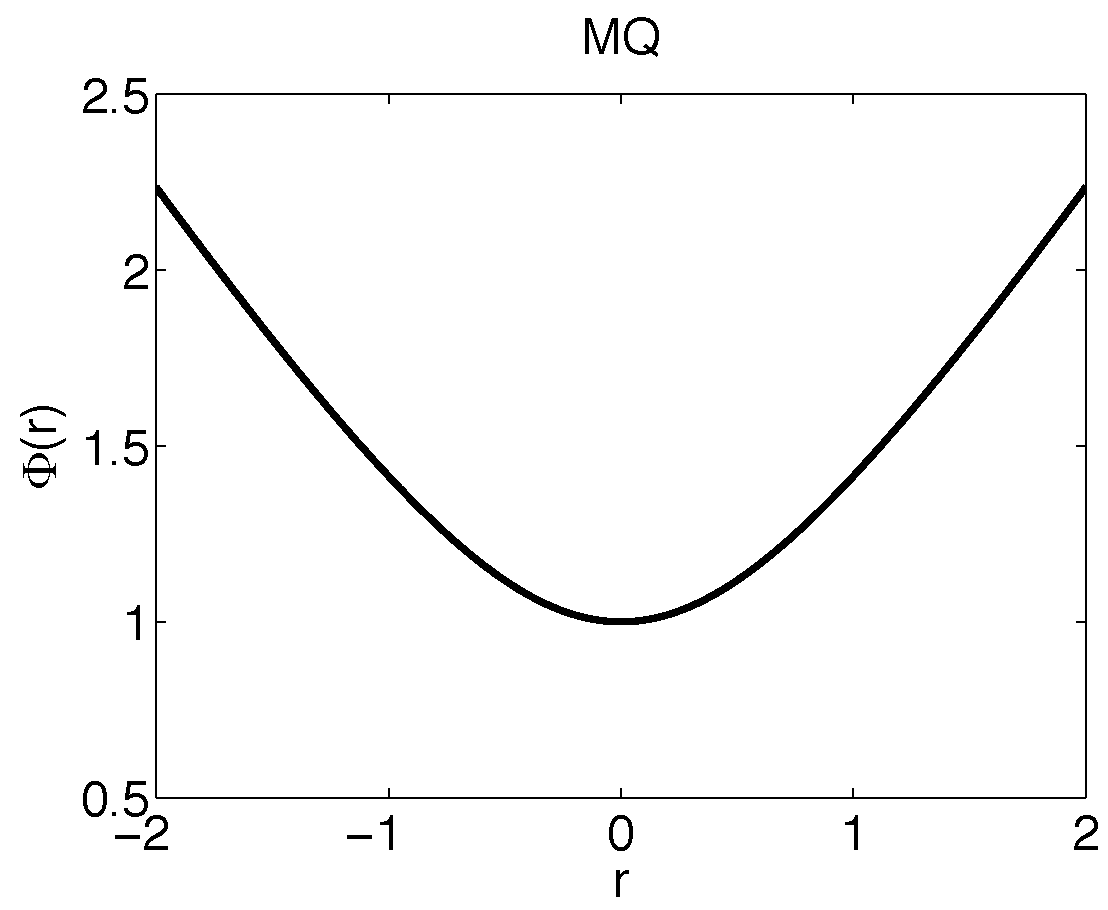
\includegraphics[width=0.25\textwidth]{matlab/mq_rbf.pdf}   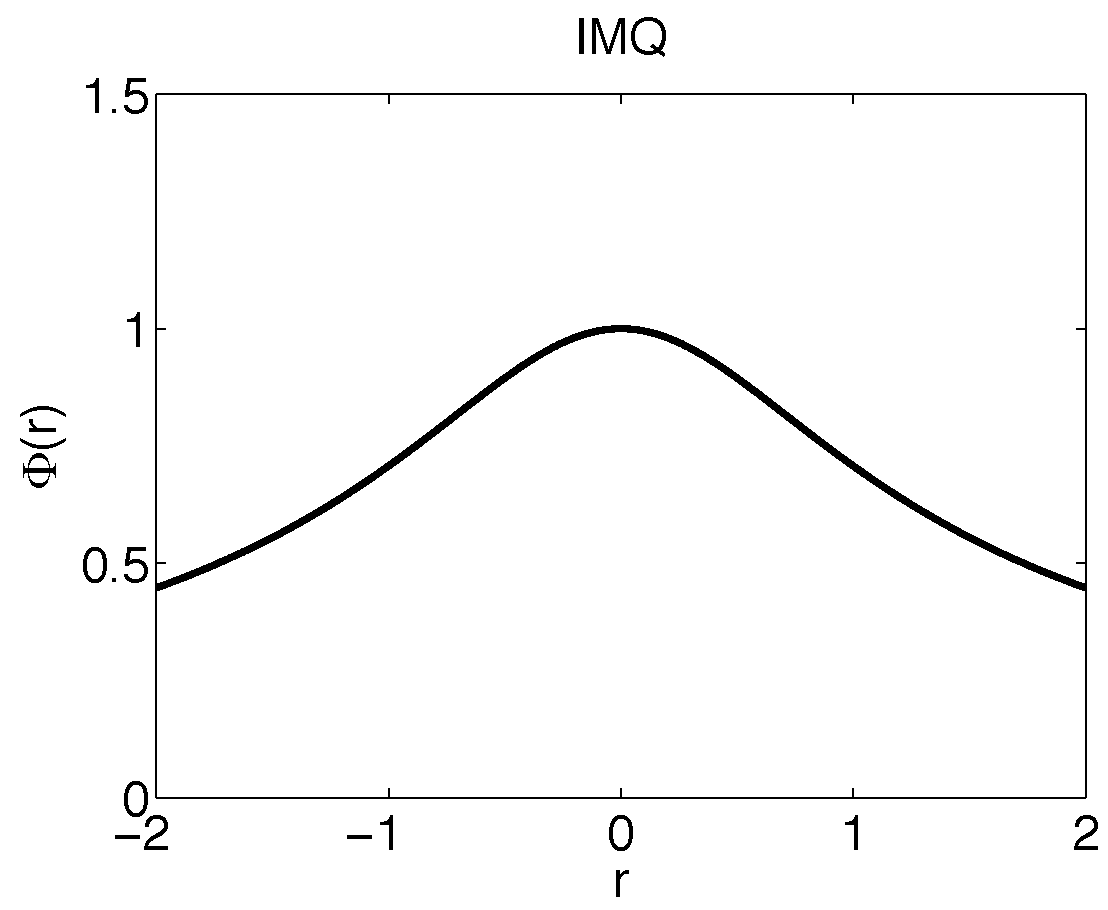
\includegraphics[width=0.25\textwidth]{matlab/imq_rbf.pdf} 
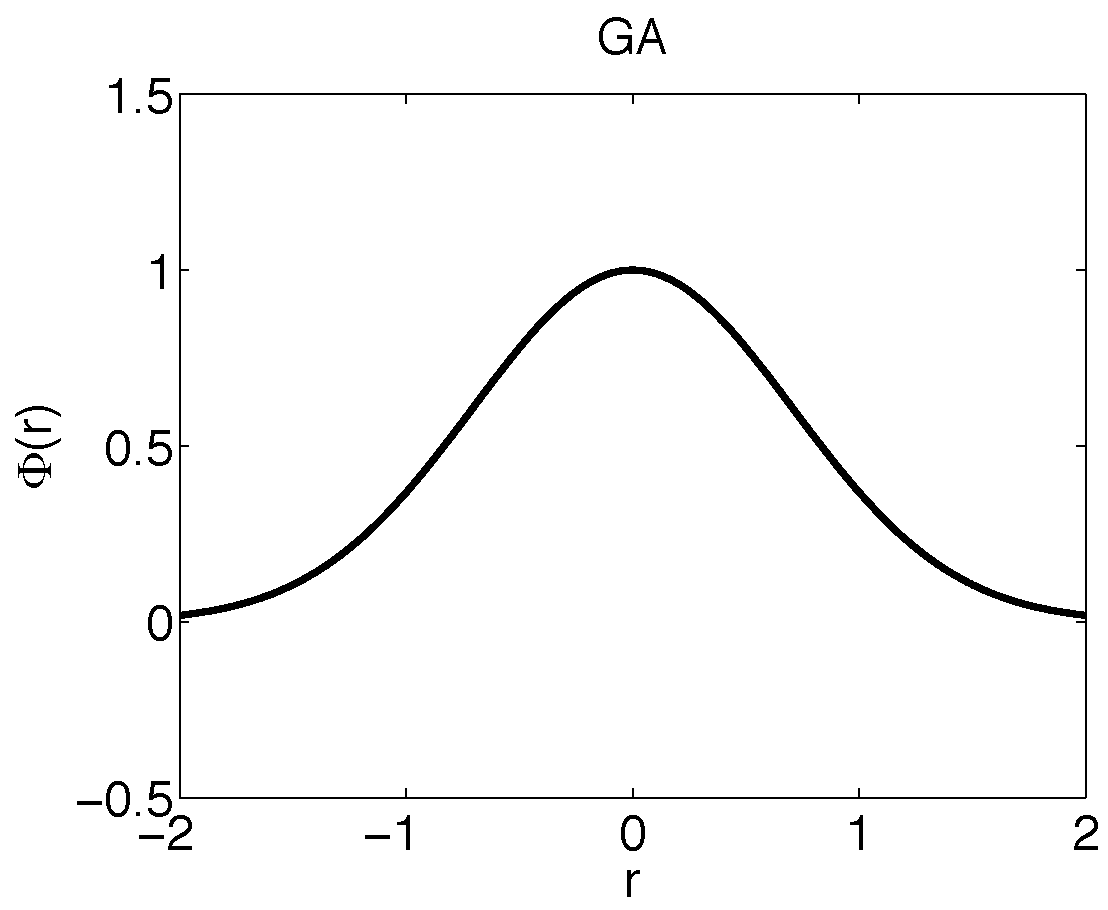
\includegraphics[width=0.25\textwidth]{matlab/ga_rbf.pdf} \\  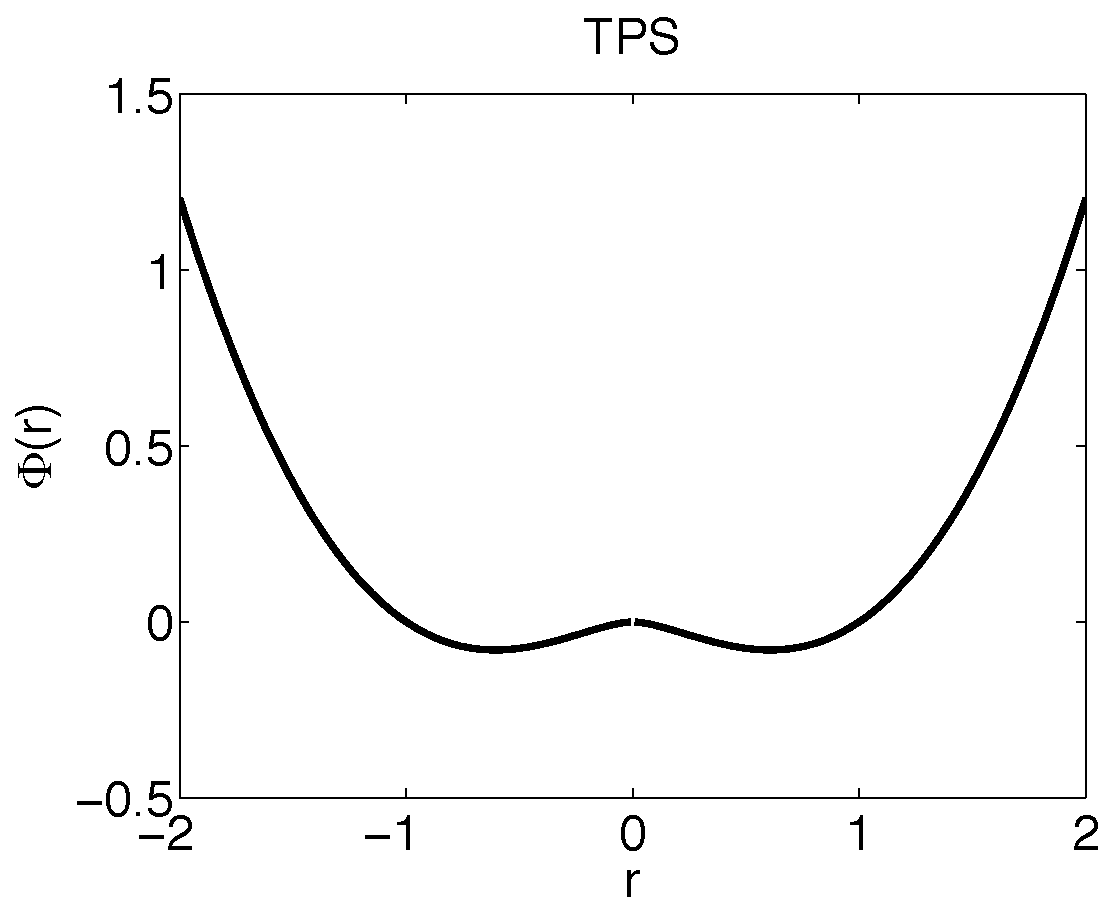
\includegraphics[width=0.25\textwidth]{matlab/tps_rbf.pdf} 
%\end{tabular} \\
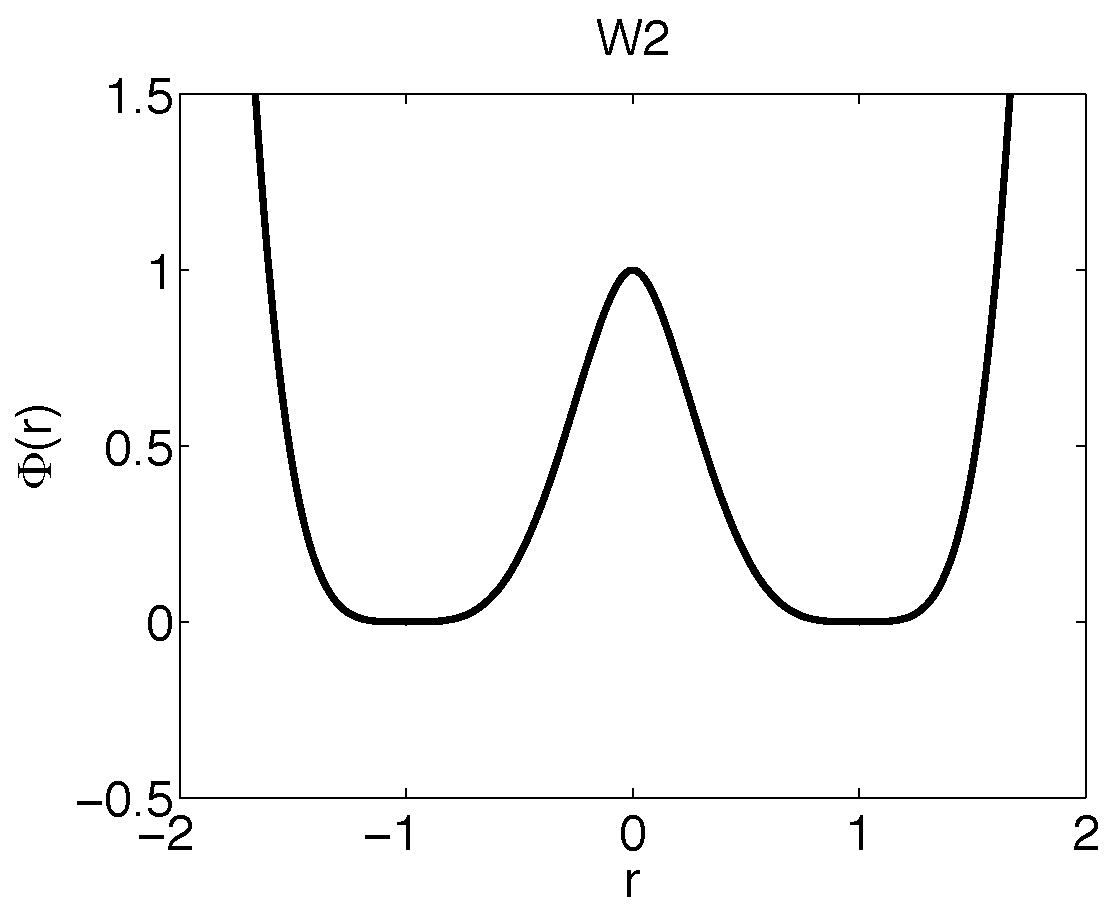
\includegraphics[width=0.25\textwidth]{matlab/w2_rbf.pdf}
\caption{Example RBF shapes from Table~\ref{tbl:rbfs} with parameter $\varepsilon=1$.}
\label{fig:rbf_examples}
\end{figure} 


\begin{figure}[t]
\centering
\begin{tabular}{cc}
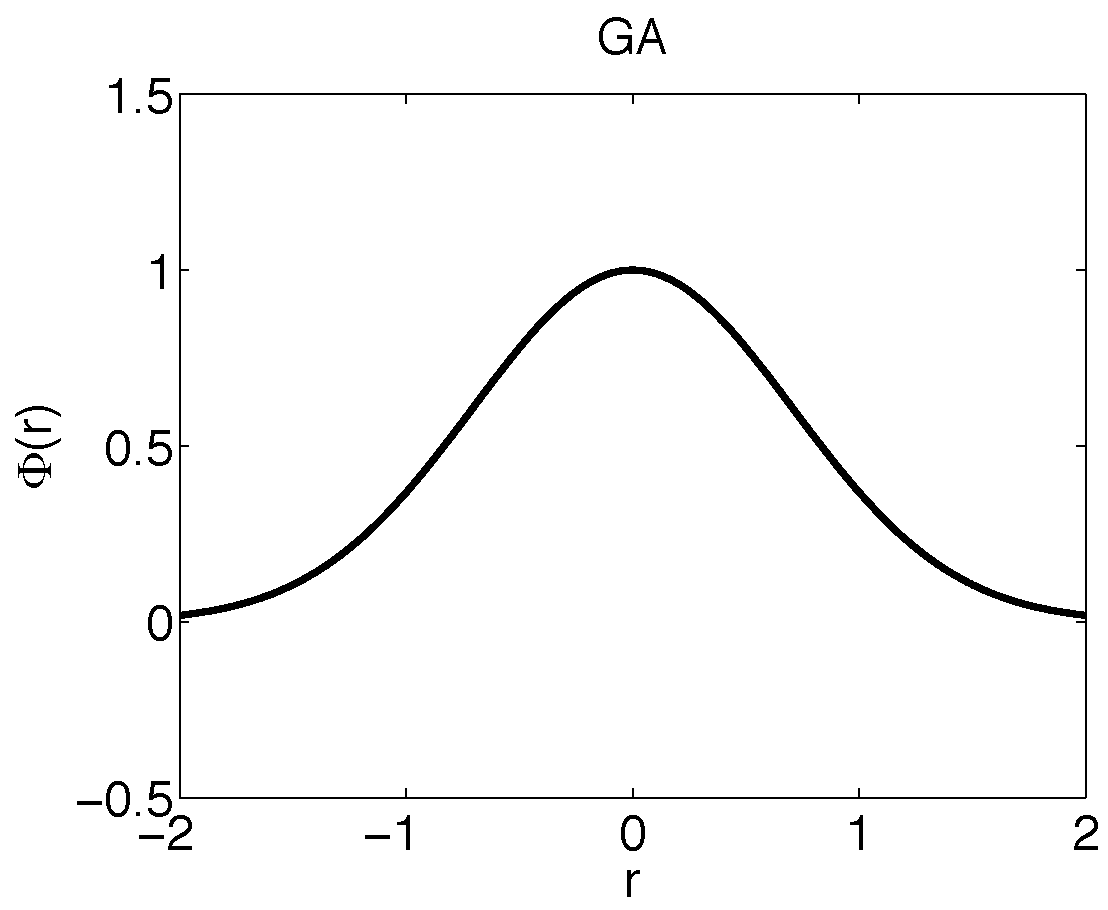
\includegraphics[width=0.25\textwidth]{matlab/ga_rbf.pdf}
\includegraphics[width=0.35\textwidth]{matlab/ga_rbf2D.eps}
\includegraphics[width=0.35\textwidth]{matlab/ga_rbf3D.eps}
\end{tabular} 
\caption{The Gaussian (GA) RBF (Table~\ref{tbl:rbfs}) with parameter $\varepsilon=1$ in dimensions 1, 2 and 3.}
\label{fig:rbf_dimension_example}
\end{figure} 

\begin{figure}[t]
    \centering
    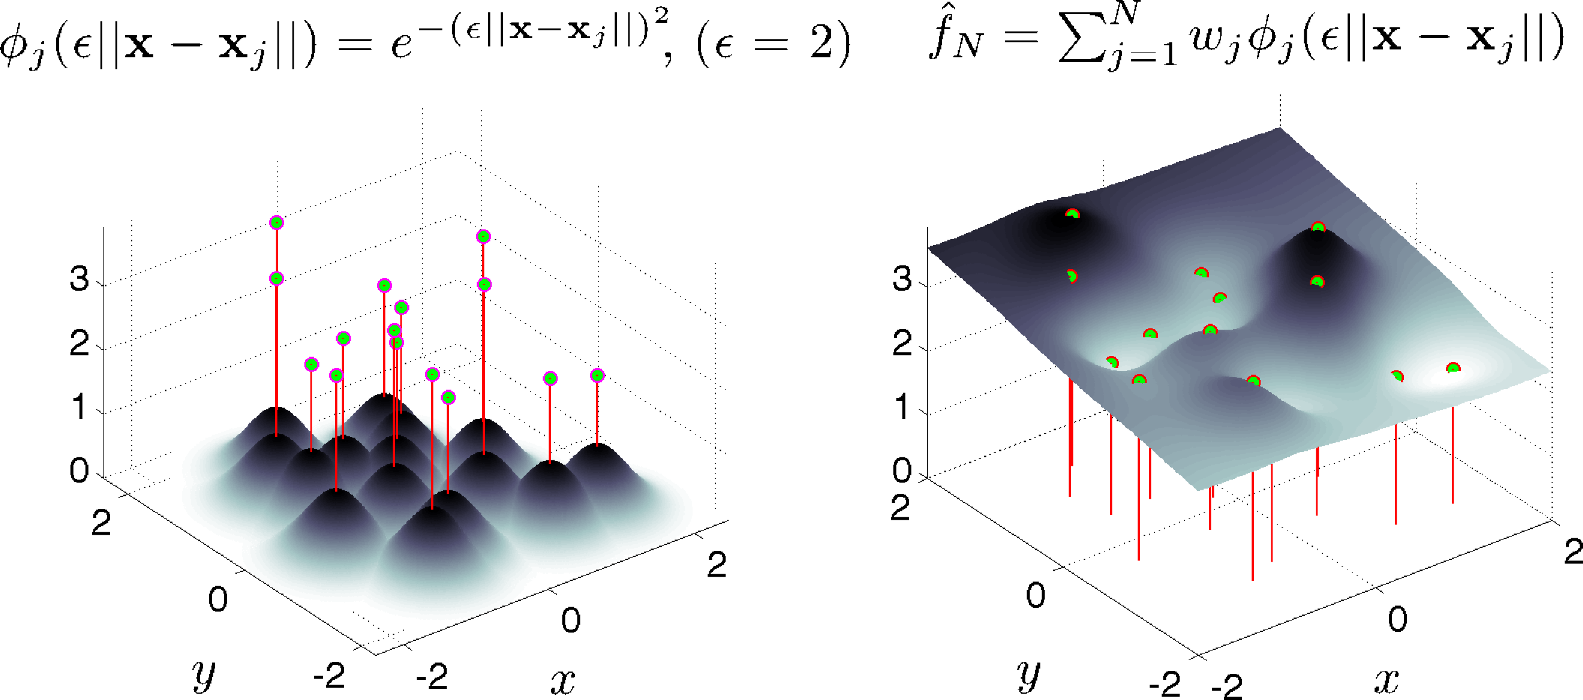
\includegraphics[scale=0.4]{figures/trimmed_interpolate2D_ga__m.pdf}
    \caption{RBF interpolation using 15 translates of the Gaussian RBF with $\epsilon=2$. One RBF is centered at each node in the domain. Linear
    combinations of these produce an interpolant over the domain passing through known function values. }
    \label{fig:rbfInterpolation}
\end{figure}

%TODO: expand with new literature since 2009
%TODO: any new methods?


RBF methods for interpolation first appeared in 1971 with Hardy's seminal research on multiquadrics
\cite{Hardy1971}. In his 1982 survey of scattered data interpolation methods \cite{Franke1982}, Franke rated multiquadrics first-in-class against 28 other methods (3 of which were RBFs) \cite{Franke1982}. Many other RBFs, 
including those presented in Table~\ref{tbl:rbfs} have been applied in literature, but for PDEs in particular, none have rivaled the 
attention received by multiquadrics. 


By 1990, the understanding of the scientific community regarding RBFs was sufficiently developed for collocating PDEs \cite{Kansa1990a,Kansa1990b}. PDE collocation seeks a solution of the form
\begin{eqnarray*}
(\diffop{u})(x_i) = \sum_{j=1}^{N} \phi_j(x_i) c_j = f(x_i)
\end{eqnarray*}
where $\diffop{}$ is, in general, a nonlinear differential operator acting on $u(x)$. The solution $u(x)$ is expressed as a linear combination of $N$ basis functions $\phi_j(x)$, not necessarily RBFs: 
$$
u(x) = \sum_{i=1}^N \phi_j(x) c_j 
$$
As in the problem of RBF scattered data interpolation, $ \vc = \{c_j\} $ is the unknown coefficient vector. 
Under the assumption that $\mathcal{L}$ is a linear operator, one can collocate the differential equation. Alternatively, individual derivative operators can be expressed as linear combinations of the unknowns $u_j$ (leading to the RBF-FD methods). 
In all cases, a linear system of equations arises, with different degrees of sparsity, dependent on the chosen basis functions and how the various constraints are enforced.  While we restrict the $\phi_j(x)$ to RBFs or various operators applied to the RBFs, we note that spectral methods, finite-element or spectral-element methods can be formulated in a similar way with different choices of basis functions.  Of course, $u$ can be a vector of unknown variables ($\vc$ then becomes a matrix). 

In Table~\ref{tbl:rbfcolloctypes} we classify references according to their choice of collocation method and RBF 
interpolation type. 
There are three main categories of RBF interpolation; we list them in Table~\ref{tbl:interp_types}. The first is \emph{Global} in the case that a single, large ($N\times N$) and 
dense matrix corresponding to globally supported RBFs is inverted; second, \emph{Compact} if compactly supported RBFs are used to 
produce a single, large, but sparse matrix; and third, \emph{Local} if compactly supported RBFs are used to produce many small but 
dense matrices with one corresponding to each collocation point. In all three cases the matrices are symmetric and with the correct choice of RBF they are at least conditionally positive definite. 

\begin{table}[t]
   \centering
   \begin{tabular}{E | C | C | C | c | } % Column formatting, @{} suppresses leading/trailing space
   Interpolation Type & Dense/Sparse $A$ & Dim($A$) ($N_S \ll N$) &  \# of $A^{-1}$  & RBF Support \\ 
   \hline \hline
   Global & Dense & $N \times N$ & 1 & Global \\
   Compact & Sparse & $N \times N$ & 1 & Compact \\
   Local & Dense & $N_S \times N_S$ & N & Global/Compact
   \end{tabular}
   \caption{RBF interpolation types and properties, assuming a problem with $N$ nodes.}
   \label{tbl:interp_types}
\end{table}


We note that three types of collocation occur throughout the RBF literature: 
Kansa's unsymmetric collocation method \cite{Kansa1990a, Kansa1990b}, Fasshauer's symmetric collocation method \cite
{Fasshauer1997}, and the Direct collocation method \cite{Fedoseyev2002}.% While not a collocation method, RBF-FD represents the latest trend in solving PDEs with RBFs.  %A full explanation of RBF based collocation is deferred to Chapter~\ref{chap:rbf_pde}. 

Prior to launching into derivation each RBF method, we first survey the classifications to highlight benefits, shortcomings, and to provide a brief historical context. A survey of related work in the RBF community that involves parallelization and optimization is deferred to Chapter~\ref{chap:parallel_rbf}. 

\subsection{Global RBF Methods}

\emph{Kansa's method} \cite{Kansa1990a, Kansa1990b} (a.k.a. unsymmetric collocation) was the first RBF method for PDEs, and is still the most frequently used method. The idea behind Kansa's method is that an 
approximate solution to the PDE can be found by finding an interpolant which satisfies the differential operator with zero residual at a set of \emph{collocation points} (these coincide with the RBF centers). To find the interpolant, the differential equation is formulated as a two block (unsymmetric) linear system with: 1) the approximation of values 
at boundary 
points with boundary data only, and 2) the approximation of interior points by directly applying the differential operator. It was 
shown in \cite{Fasshauer1997, Hon2001} that the unsymmetric linear system produced by Kansa's method does not guarantee 
non-singularity; although it is also noted that in practice singularities are rare encounters \cite{Larsson2003}. 

The second alternative for RBF collocation, is based on Hermite scattered 
data interpolation (see \cite{Wu1992}). The so-called \emph{Fasshauer} or \emph{Symmetric Collocation} method (\cite{Fasshauer1997}) 
performs a change of basis for the interpolant by directly applying the differential operator to the RBFs. It then collocates using the same approach as Kansa's method \cite{Stevens2009b, Larsson2003}. The resulting block structure of the linear system is symmetric and 
guaranteed to be non-singular \cite{Fasshauer1997}. In comparison to Kansa's method, the disadvantages of Fasshauer's method 
include: a) requirement of higher order differentiability of the basis functions (to satisfy double application of the differential operator)
% it has stronger regularity assumptions (it is Hermite interpolation), 
and b) the linear system is larger and more complex to form
%, and c) it is not ideally suited for non-linear problems
 \cite{Fasshauer2007}. As \cite{Hon2001} points out, 
the possible existence of a singularity in Kansa's method is not enough to justify the added difficulties of using Fasshauer's 
method.

%TODO: refs that refer to global RBF methods and RBF-PS as just RBF methods. 

The last collocation method, \emph{Direct Collocation}, was introduced by Fedoseyev, Friedman and Kansa
 \cite{Fedoseyev2002} and satisfies the differential operator on the interior and the boundary. Larsson and Fornberg \cite{Larsson2003} observe that this third method has a matrix structure similar to that found in Kansa's method; however, it is noted that the dimensions of the matrix blocks for each method differ. This is due to collocation constraints added for 
the differential operator applied to the boundary. Aside from the survey on RBF collocation presented by Larsson and Fornberg \cite{Larsson2003}, no related 
work was found that applied, or investigated, this method further.  

Both Kansa's method and Fasshauer's methods were shown in \cite{Fasshauer2006} to fit well in the generalized framework of pseudo-spectral methods with a subtle change in algorithm. While collocation methods explicitly compute the coefficients for a continuous derivative approximation, their alternates, referred to in literature as RBF-pseudospectral (RBF-PS) methods, never explicitly compute the interpolant coefficients. Instead, a differentiation matrix (DM) is assembled and used to approximate derivates at the collocation points only \cite{FasshauerZhang2007}. Since most computational models are simply concerned with the solution at collocation points, the change to assemble DMs as in RBF-PS is organic. 


Following the evolution of the RBF-PS algorithm, applications of global RBFs in the classic collocation sense (i.e., without the RBF-PS DMs) become impractical. This statement stems from the algorithmic complexity of each method. 
%As discussed in \cite{Fasshauer2007, FlyerWright09}, RBF methods result in matrices that are full. The 
Global RBF methods result in full matrices \cite{Fasshauer2007}. The global collocation methods then scale on the order of $O(N^3)$ floating point operations (FLOPs) to solve for weighting coefficients on a given node layout, plus $O(N^2)$ to apply the weights for derivatives. If time-stepping is required, global collocation methods must recompute the time-dependent coefficients with additional cost dominated by $O(N^3)$ operations. RBF-PS methods have similar requirements for $O(N^3)$ operations to assemble the differentiation matrix and $O(N^2)$ to apply for derivatives. However, by avoiding time-dependent coefficients, RBF-PS methods only apply the differentiation matrix each time-step for $O(N^2)$ operations. As an aside, the $O(N^3)$ complexity for each method---typically due to an LU-decomposition, with subsequent forward- and back-solves---could be reduced. While not in mainstream use by the RBF community, \cite{Morse2005} correctly points out that the use of iterative solvers could reduce complexity of preprocessing to the order of $O(N^2)$. 
%For mid- to large-scale problems, in the unlikely event that conditioning of the system is not a limiting factor, the cost of the method is still seen as prohibitively high. 

Hon et al. \cite{Hon1999} employed Kansa's method to solve shallow water equations for Typhoon simulation.
In \cite{FlyerWright09}, Flyer and Wright employed RBF-PS (Kansa method) for the solution of shallow water equations on a sphere. Their 
results show that RBFs allow for longer time steps with spectral accuracy. The survey \cite{FlyerFornberg11} by Flyer and Fornberg showcases RBF-PS (Kansa) out-performing some of the of the best available methods in geosciences, namely: Finite Volume, Spectral Elements, Double Fourier, and Spherical Harmonics. When applied to problems such as transport on the sphere \cite{FlyerWright07}, shallow water equations \cite{FlyerWright09}, and 3D mantle convection\cite{WrightFlyerYuen10}, RBF-PS consistently required fewer time steps, and a fraction of the nodes for similar accuracy \cite{FlyerFornberg11}. 
%TODO: add \cite{Neves2009}

%
%In the survey on RBF collocation presented by Larsson and Fornberg \cite{Larsson2003}, it was found that performance of the 
%collocation methods depends on the choice of RBFs (i.e., whether they are infinitely smooth or piecewise smooth). Their end 
%conclusion, however, was that infinitely smooth RBFs are preferred for Elliptic PDEs as they do not require node placement 
%optimization.

%Kansa collocation
\newcommand{\kansaglobalrbf}[0]{\cite{Kansa:1990a, Kansa:1990b, Fasshauer:2006, Fornberg:2004, Mouat:2002, Hon:2001, Franke:1982, Flyer:2009b, Flyer:2007, Hon:1999, Fornberg:2008, Larsson:2003}}
\newcommand{\kansacsrbf}[0]{\cite{Fornberg:2008, Wang:2002}}
\newcommand{\kansalocalrbf}[0]{\cite{Divo:2007, Kosec:2008, Sarler:2006, Vertnik:2006}}

% Fasshauer collocation
\newcommand{\fassglobalrbf}[0]{\cite{Fasshauer:2006, Fasshauer:1997, Larsson:2003}}
\newcommand{\fasscsrbf}[0]{\cite{Liu:2005}}
\newcommand{\fasslocalrbf}[0]{\cite{Stevens:2008a, Stevens:2009a, Stevens:2009b}}

% Direct collocation
\newcommand{\directglobalrbf}[0]{\cite{Fedoseyev:2002, Larsson:2003}}
\newcommand{\directcsrbf}[0]{}
\newcommand{\directlocalrbf}[0]{}


% RBF-FD
\newcommand{\rbffdglobalrbf}[0]{N/A}
\newcommand{\rbffdcsrbf}[0]{N/A}
\newcommand{\rbffdlocalrbf}[0]{\cite{Wright:2006,Wright:2003, Shu:2003, Cecil:2004, Wright:2004, Shu:2006, Chandhini:2007}}


%\begin{sidewaystable}
\begin{table}[t]
\begin{center}
	\begin{tabular}{@{} R|C|C|C|}
		& \multicolumn{3}{c|}{RBF Interpolation Type} \\
		\hline
		Method & Global (Dense) & Compact (Sparse Global) & Local \\
		\hline \hline
		Kansa's Method &\kansaglobalrbf & \kansacsrbf & \kansalocalrbf \\
		\hdashline
		Fasshauer's Method &\fassglobalrbf & \fasscsrbf & \fasslocalrbf \\
		\hdashline
		Direct Collocation &\directglobalrbf & \directcsrbf & \directlocalrbf \\
		\hdashline
		RBF-FD & \rbffdglobalrbf & \rbffdcsrbf & \rbffdlocalrbf \\
		\hline
	\end{tabular}
\end{center}
\caption{Classification of references based on choice of RBF interpolation types and method for solving PDEs. References may appear in multiple cells according to the breadth of their research.}
\label{tbl:rbfcolloctypes}
\end{table}
%\end{sidewaystable}




\subsection{Compactly Support RBFs} 

Thus far, all cases of collocation and interpolation mentioned have assumed globally supported RBFs. While global RBFs are well-studied and have nice properties, a major limitation is the large, dense system that must be solved. One alternative to global support is to use a set of compactly supported RBFs (CSRBFs) that are defined as: 
\begin{equation}
\phi(r) = \begin{cases} \varphi(r) & r \in [0,1]\\
0 & r > 1
\end{cases}
\label{eqn:csrbf}
\end{equation}
where a radius is defined past which the RBF (in this case $\varphi(r)$) has no influence on the interpolant. Note that the radius can be scaled to fit a desired support. Methods that leverage CSRBFs produce a global interpolation matrix that is \emph{sparse} and therefore results in a system that is more efficiently assembled and solved \cite{Fasshauer2007}. The actual complexity estimate of the CSRBF method depends on the sparsity of the problem as well as the ordering of the assembled system. Assuming $n \ll N$ where $n$ represents the number of nodes in support, \cite{Zhang2004} approximates the complexity as dominated by $O(N)$ for properly structured systems within MATLAB, and the investigation in \cite{Morse2005} found $O(N^{1.5})$ consistent with the estimate provided by their choice of general sparse solver package. Fasshauer \cite{Fasshauer2007} provides a stationary multilevel collocation method based on CSRBF with $O(N)$ complexity, but the method is plagued by poor convergence. In the context of CSRBFs, analogues to Kansa's method and Fasshauer's method are known by the names \emph{radial point interpolation method (RPIM)} \cite{Wang2002} and \emph{radial point interpolation collocation method (RPICM)} \cite{Liu2005}, respectively. A more thorough survey of CSRBF history can be found in \cite{Fasshauer2007,Iske2004}.

CSRBFs have attracted a lot of attention in applications. For example, in the field of dynamic surface and image deformation, compact support allows for local transformations which do not induce global deformation (see e.g., \cite{Yang2008, Lin2009, Correa2007}). 

We note that sparsity and spectral accuracy cannot be achieved simultaneously. 


\subsection{Local RBF Methods}
% TODO: review these papers
Around 2005, \v{S}arler and Vertnik \cite{Sarler2006, Vertnik2006} demonstrated that if compactly supported RBFs are chosen, the traditional global 
collocation matrix from Kansa's method, can be avoided altogether in favor of small localized collocation matrices defined for 
each node. Local collocation still faces possible ill-conditioning and singularities 
like global collocation, but make it easier to distribute computation across parallel systems. Also, the smaller linear systems can be 
solved 
with less conditioning issues. In \cite{Sarler2006}, the authors consider 2D diffusion problems. Divo and Kassab \cite{Divo2007} 
employ the 
method for Poisson-like PDEs including fluid flow and heat transfer. Kosec and \v{S}arler \cite{Kosec2008} apply the 
same technique to solve coupled heat transfer and fluid flow problems.

In similar fashion, Stevens et al. \cite{Stevens2009a} introduced a local version of 
Fasshauer's method called \emph{local Hermitian interpolation}. The authors have applied their method to 3D soil 
problems based on transient Richards' equations \cite{Stevens2008a, Stevens2009a, Stevens2009b}.


\subsection{Recent Advances in Conditioning}

Recently, Fornberg and Wright 
\cite{Fornberg2004} presented the \emph{Contour--Pad\'{e} algorithm}, which allows for numerically stable 
computation of highly 
accurate interpolants for (very small) cases typically associated with ill-conditioning induced by nearly flat RBFs (i.e., $\epsilon \rightarrow 0$). Larsson and Fornberg \cite{Larsson2003} 
applied the 
algorithm to all three methods of collocation (Kansa's, Fasshauer's and Direct Collocation) with considerable gain in accuracy over solutions from classical second-order FD and a pseudospectral method. Note that currently, the Contour-Pad\'{e} 
algorithm was only studied for global RBF interpolation, not for compact or local methods. 

The \emph{RBF-QR} method, an alternative for numerically stable computation in the limit as $\epsilon \rightarrow 0$, was introduced by Fornberg  and 
Piret \cite{Fornberg2007} in context of a sphere, and later extended to planar 2D problems in \cite{Fornberg2009b}. The 
RBF-QR 
method is simple 
to implement (less than 100 lines of Matlab code), and it allows solution of large problems that are typically ill-conditioned. Fornberg, Larsson and Flyer \cite{Fornberg2009b} successfully applied RBF-QR on large problems with 6000 nodes for globally supported basis functions. 
%TODO: add mention of bengt's latest on RBF-QR \cite{Fornberg2011a, Fornberg2011b}

With these two algorithms, global RBF methods have overcome most ill-conditioning issues for small to mid-sized problems. Unfortunately, both Contour-Pad\'{e} and RBF-QR fail for large enough problems due to ill-conditioning. As the number of RBFs increases beyond a few thousand nodes it is impossible to avoid  ill-conditioning of the extremely large interpolation matrix.

This reveals the benefit of local methods, which decrease the number of RBFs and ill-conditioning. However, in the limit as local stencil size increases to include all nodes in a domain, the local and global method are equivalent; thus it is known that local methods also suffer extreme ill-conditioning around 2000 nodes per stencil \cite{Shu2006}. To our our knowledge, no research has yet been published that applies the RBF-QR method to RBF-FD stencils.

%
%In 2002, Mouat and Beatson \cite{Mouat2002} suggested that Matern functions would be more accurate than the more 
%commonly chosen multiquadrics. 
%The authors also considered the problem of a large number of nodes with a discussion of a 
%domain decomposition method for PDE solution. 


% TODO: add partition of unity discussion


\section{Comparison of RBF Methods}

We now detail RBF methods for PDEs leading up to the derivation of RBF-FD. 

Following \cite{Mouat2002}, consider a PDE expressed in terms of a (linear) differential operator, $\diffop$: 
\begin{eqnarray*}
\diffop{u} & = & f \on{\Interior} \\
u &=& g \on{\Boundary}
\end{eqnarray*}
where $\Interior$ is the interior of the physical domain, $\Boundary$ is the boundary of $\Interior$ and $f,g$ are known explicitly. In the case of a non-linear differential operator, a Newton's iteration, or some other method, can be used to linearize the problem (see e.g., \cite{WrightFornberg06}); of course, this increases the complexity of a single time step. Then, the unknown solution, $u$, which produces the observations on the right hand side can be approximated by an interpolant function $u_{\phi}$ expressed as a linear combination of radial basis functions, $\{\phi_j(x) = \phi(\vectornorm{x-x_j})\}_{j=1}^{N}$, and polynomial functions$\{P_l(x)\}_{l=1}^{M}$:
\begin{equation}
	u_{\phi}(x) = \sum_{j=1}^{N}  \phi_j(x) c_{j} + \sum_{l=1}^{M}  P_l(x) d_{l}, \hskip1.5em P_l(x) \in \Pi^{D}_{p}
	\label{eqn:pde_approx}
\end{equation}
where $\phi_j(x) = \vectornorm{x - x_j}$ ($\vectornorm{\cdot}$ is standard Euclidean distance). The 
second sum represents a linear combination of polynomials that enforces zero approximation error
 when $u(x)$ is a polynomial of degree less than or equal to $p$. The variable $D$ is the 
 problem dimension (i.e., $u_{\phi}(x) \in \R^{D}$). 
%\toevan{Finish to end of paragraph} 
To eliminate degrees of freedom for well-posedness, $p$ should be greater than or equal to the order of the chosen RBF
 (see Table~\ref{tbl:rbfs}) \cite{Iske2004}.  
Note that Equation~\ref{eqn:pde_approx} is evaluated 
 at $\{x_j\}_{j=1}^{N}$ 
data points through which the interpolant is required to pass with zero residual.  We refer to 
the $x_j$'s as \emph{collocation points} (a.k.a. trial points), taken as the RBF centers. The test points, $x$, usually coincide with collocation points, although this is not a requirement. 
%$P_l(x)$ is needed to eliminate degrees of freedom for well-posedness \cite{Iske:2004}. 

To clarify the role of the polynomial part in Equation~\ref{eqn:pde_approx}, it is necessary to
put aside the PDE for the moment and consider only the problem of \emph{scattered data 
interpolation} with Radial Basis Functions.

\subsection{RBF Scattered Data Interpolation}
 Borrowing notation from \cite{Fasshauer2007, Iske2004}, 
we seek an interpolant of the form
\begin{eqnarray*}
f(x) = \sum_{j=1}^{N} \phi_j(x) c_{j}  \label{eq:rbf_scattered_data_interp}
\end{eqnarray*}
where $f(x)$ is expressed as a scalar product between the unknown coefficient weights $c_j$ and the radial basis functions $\phi_j(x)$.

To obtain the unknown coefficients, $c_j$, form a linear system in terms of the $N$ RBF centers:
\begin{eqnarray*}
f(x) & = & \sum_{j=1}^{N} c_{j}  \phi_j(x)  \hskip1.5em \textrm{for\ } x = \{x_j\}_{j = 1}^{N} \\
 \parray{c}{ f } & =&  \barray{c}{\phi}\parray{c}{ c } 
\end{eqnarray*}
The invertibility of this system depends on the choice of RBF, so one typically chooses a function that is positive definite to avoid issues. It has been shown (see \cite{Fasshauer2007, Iske2004}) that some choices of RBFs (e.g. multiquadrics and thin-plate splines \cite{Hon2001}) are not positive definite and therefore there is no guarantee that the approximation is well-posed. A sufficient condition for well-posedness is that the matrix be \emph{conditionally positive definite}. In \cite{Fasshauer2007}, Fasshauer demonstrates that conditional positive definiteness is guaranteed when Equation~\ref{eqn:pde_approx} exactly reproduces functions of degree less than or equal $m$. 
For RBF scattered data interpolation in one dimension, this can be achieved by adding a polynomial of order $m$ with $M =$${m+1}\choose{1}$ terms (e.g., $x^0, x^1, \cdots, x^{m}$). For $\R^2$, the terms would be: $1, x, y, xy, x^2y, xy^2, \cdots, x^{m}y^{m-1}, x^{m-1}y^{m}, x^my^m$. In $\R^D$, $M =$${m+D}\choose{D}$ \cite{Iske2004}, giving
\begin{eqnarray}
\sum_{j=1}^{N} c_{j}  \phi_j(x)  +  \sum_{l=1}^{M} d_{l} P_l(x) & = & f(x),  \hskip1.5em  P_l(x) \in \Pi^{D}_{m} \label{eq:interpolation_constraints} \\
\left[ \begin{array}{c c} 
	\phi & P
	\end{array} \right] \left( \begin{array}{c}
							c \\
							d
							 \end{array}
						 \right) & = & \parray{c}{ f } \nonumber
\label{eqn:interpolation_constraints}
\end{eqnarray}
where the second summation (referred to as \emph{interpolation conditions} \cite{Iske2004}) ensures the minimum degree of the interpolant. Refer to Table~\ref{tbl:rbfs} for a short list of recommended RBFs and minimally required orders of $m$. This document prefers the Gaussian RBF. Notice, in Equation~\ref{eq:interpolation_constraints}, that the interpolation conditions add $M$ new degrees of freedom, so we must provide $M$ 
additional constraints to square the system. In this case:
$$
\sum_{j=1}^{N} c_{j} P_l(x_j) = 0,  \hskip1.5em  l=1,..., M 
$$
or 
\begin{eqnarray}
P^T {c}  = {0}. 
\label{eqn:extra_constraints}
\end{eqnarray}
It is now possible again to write the interpolation problem as a linear system using Equations~\ref{eqn:interpolation_constraints} and \ref{eqn:extra_constraints}:%as
\begin{eqnarray}
 \underbrace{\left[ \begin{array}{c c} 
	\phi & P \\
	P^T & 0
	\end{array} \right]}_{A_{\diffop{}}} \left( \begin{array}{c}
							c \\
							d
							 \end{array}
						 \right) = \left( \begin{array}{c}
							f \\
							0
							 \end{array}
						 \right) \label{eq:solve_rbf_scattered_interp}
\end{eqnarray}
%This system then produces coefficients capable of exactly approximating data from polynomials of degree less than or equal to $m$ \cite{Fasshauer2007}. 
Equation~\ref{eq:solve_rbf_scattered_interp}, typically a dense system except in the case of RBFs with compact support, can be solved efficiently via standard methods like LU-decomposition.  With the coefficients, the interpolant can be sampled at any test points, $\{x_i\}_{i=1}^{n}$, by returning to Equation~\ref{eq:rbf_scattered_data_interp}:
\begin{eqnarray}
f(x_i) & = & \sum_{j=1}^{N} c_{j}  \phi_j(x_i) +  \sum_{l=1}^{M} d_{l} P_l(x_i)  \\
 & = & \left. \underbrace{\left[ \begin{array}{c c} 
       \phi &  P
	\end{array} \right]}_{B} 
	  \left( \begin{array}{cc}  c \\ d  \end{array} \right) \ \right|_{x={x_i}}
	\label{eqn:interpolate_x}
\end{eqnarray}


\subsection{Reconstructing Solutions for PDEs}
In the next few subsections, we will consider collocation equations based on this general form: 
\begin{eqnarray*}
\diffop{u_\phi(x)} &=& f(x) \on{\Interior} \label{eqn:colloc_interior}\\ 
\boundop{u_\phi(x)} &=& g(x) \on{\Boundary}  \label{eqn:colloc_boundary} 
\end{eqnarray*}
where the methods presented below will apply the differential operators, $\diffop{}$ and $\boundop{}$, to different choices of $u_\phi$ and different sets of collocation points. In many applications $\diffop{}$ is chosen as a differential operator (e.g., $\pd{}{x}$, $\nabla$, $\nabla^2$) and $\boundop = I$ (i.e. identity operator for Dirichlet boundary conditions) for PDEs. For RBF scattered data interpolation, $\diffop{} = I$. There are also  applications where $\diffop{}$ is a convolution operator (see e.g., \cite{Carr2001, Carr2003}) capable of smoothing/de-noising a surface reconstructed from point clouds. 

%TODO: label x_j's as TRIAL and x_is as TEST points
%\section{Approximating the Solution}
For all the methods to be presented a linear system is generated: 
$$
A_{\diffop{}}  \left( \begin{array}{cc}  c \\ d  \end{array} \right)  =  \left( \begin{array}{cc}  f \\ 0  \end{array} \right) 
$$
\begin{equation}
  \left( \begin{array}{cc}  c \\ d  \end{array} \right) = A^{-1}_{\diffop{}}  \left( \begin{array}{cc}  f \\ 0  \end{array} \right)
  \label{eqn:solve_coeffs}
 \end{equation}
 where matrix $A_{\diffop{}}$ depends on the choice of collocation method. 
Once the linear system is solved, the value $u(x)$ is reconstructed at the test points following Equation~\ref{eqn:interpolate_x}:
\begin{eqnarray}
u(x) & = &  \left.
\left[ \begin{array}{c c} 
       \phi &  P
	\end{array} \right]
	  \left( \begin{array}{cc}  c \\ d  \end{array} \right)  \ \right|_{x={x_i}} \nonumber\\
	 & = & B A^{-1}_\diffop{} \left( \begin{array}{cc}  f \\ 0  \end{array} \right) 
	\label{eqn:solve_u}
\end{eqnarray}
Likewise, to obtain differential quantities we have: 
\begin{eqnarray*}
\diffop{u}(x) & = & \left.
\left[ \begin{array}{c c} 
       \diffop{\phi} &  \diffop{P}
	\end{array} \right]
	  \left( \begin{array}{cc}  c \\ d  \end{array} \right)  \ \right|_{x={x_i}} \\
  	 & = & B_{\diffop{}} A^{-1}_\diffop{} \left( \begin{array}{cc}  f \\ 0  \end{array} \right).
	\label{eqn:solve_uxx}
\end{eqnarray*}

%Here we substitute $B$ for test samples in Equation~\ref{eqn:solve_u} to get the reconstructed solution:
%\begin{eqnarray}
%u(x) = B A^{-1}_\diffop{} \left( \begin{array}{cc}  f \\ 0  \end{array} \right)
%	\label{eqn:solve_rbf}
%\end{eqnarray}
%where the vector-matrix inner product $(A A^{-1}_{\diffop{}})$ is a row-vector. Since the coefficient vectors ${c}$ and ${d}$ are the same for all $x_i$, we can group the evaluation of $\diffop{u(x_i)}$ for $i=1,...,n$ as a matrix-vector multiplication where the matrix rows correspond to $(A_\diffop{} A^{-1})$ for each $x_i$. 


%TODO: mention equation~\ref{eqn:solve_rbf} can be precomputed DM applied to f for collocation points in pseudo-spectral method.  
%Relevant to the discussion of RBF-PS and computational and memory efficient global RBF methods, if $A$ contains rows corresponding to the interpolation problem can be rewritten independent of coefficients by assembling a differentiation 

\subsection{PDE Methods} 

Now, since $u_{\phi}(x)$ from Equation~\ref{eqn:pde_approx} cannot (in general) satisfy the PDE everywhere, we enforce the PDE at a set of collocation points, which are  distributed over both the interior and the boundary. Again, these points do not necessarily coincide with the RBF centers, but it is convenient for this to be true in practice. 

\subsubsection{Kansa's Method}

The first global RBF method for PDEs, \emph{Kansa's method} \cite{Kansa1990a, Kansa1990b}, collocates the solution through known values on the boundary, while constraining the interpolant to satisfy the PDE operator on the interior. This is equivalent to choosing $u_\phi$ according to Equation~\ref{eqn:pde_approx}. The resulting system is given by \cite{Mouat2002}; assuming that $\diffop{}$ is a linear operator, 
\begin{eqnarray}
\diffop{u_\phi(x_i)} = \sum_{j=1}^{N}c_j\diffop{\phi_j(x_i)} + \sum_{l=1}^{M}d_l \diffop{P_l(x_i)} &=&f(x_i)  \hskip1.5em i = 1,...,n_I  \label{eqn:kansa_interior} \\ 
\boundop{u_\phi(x_i)} = \sum_{j=1}^{N}c_j \boundop{\phi_j(x_i)} + \sum_{l=1}^{M}d_l \boundop{P_l(x_i)} &=& g(x_i)  \hskip1.5em i = n_I + 1, \cdots, n \label{eqn:kansa_boundary} \\
\sum_{j=1}^{N} c_j P_l(x_j) & = & 0 \hskip3.0em l=1,\cdots,M \label{eqn:kansa_constraints} 
\end{eqnarray}
where $n_I$ are the number of interior collocation points, with the number of boundary collocation points equal to $n - n_I$. First, observe that the differential operators are applied directly to the RBFs inside summations, rather than first solving the scattered data interpolation problem and then applying the operator to the interpolant.  Second, since the basis functions are known analytically, it is possible (although sometimes painful) to derive $\diffop{\phi}$ (refer to \cite{Fasshauer2007} for RBF derivative tables); the same is true for the polynomials $P_l$. 

We can now reformulate Kansa's method as the linear system: 
\begin{eqnarray}
\underbrace{\left[ \begin{array}{c c} 
	\phi_\diffop{} & P_\diffop{} \\
	\phi_\boundop{} & P_\boundop{} \\
	P^T & 0
	\end{array} \right]}_{A_{\diffop{}}}  \left( \begin{array}{c}
							{c} \\
							{d}
							 \end{array}
						 \right) = \left( \begin{array}{c}
							{f} \\
							{g} \\
							0
							 \end{array}
						 \right) 
	\label{eqn:kansa_method}
\end{eqnarray}
% TODO: add underline stating that matrix is A. 


where $\phi_\diffop{} = \diffop{\phi}$, $P_\diffop{} = \diffop{P}$ are the interior components (Equation~\ref{eqn:kansa_interior}), $\phi_\boundop{}$ and $P_\boundop{}$ are the boundary components (Equation~\ref{eqn:kansa_boundary}), and $P^T = \left[P_\diffop{}^T \ \ P_\boundop{}^T\right]$ are constraints for both interior and boundary polynomial parts (Equation~\ref{eqn:kansa_constraints}). From Equation~\ref{eqn:kansa_method} it should be clear why Kansa's method is also known as the \emph{Unsymmetric} collocation method. 

%\toevan{Isn't $N+M=n$? For each case, you must put the proper relationships between $N$, $M$, $n_I$, $n$ so that the number of constraints equals the number of relations.}
Recall that the matrix in Equation~\ref{eqn:kansa_method} has no guarantee of non-singularity \cite{Fasshauer1997}; however, singularities are rare in practice \cite{Larsson2003}. 

\subsubsection{Fasshauer's Method}

\emph{Fasshauer's method} \cite{Fasshauer1997} addresses the problem of singularity in Kansa's method by assuming the interpolation to be Hermite. That is, it requires higher differentiability of the basis functions (they must be at least $C^k$-continuous if $\diffop{}$ is of order $k$). Leveraging this assumption, Fasshauer's method chooses: 
\begin{eqnarray}
u_\phi(x_i) & = & \sum_{j=1}^{N_I}  c_j \diffop{\phi_j(x_i)} + \sum_{j=N_{I} + 1}^{N} c_j \boundop{\phi_j(x_i)} + \sum_{l=1}^{M}d_l P_l(x_i)
\label{eqn:fasshauer_approx}
\end{eqnarray}
as the interpolant passing through collocation points. Note $N_I$ is used here to specify the number of RBF centers in the interior of $\Omega$. Here the interpolant is similar to Equation~\ref{eqn:pde_approx}, but a change of basis functions is used for the expansion: $\diffop{\phi_j(x)}$ on the interior and $\boundop{\phi_j(x)}$ on the boundary.

Collocating (i.e., substituting Equation~\ref{eqn:fasshauer_approx} into Equations~\ref{eqn:kansa_interior}-\ref{eqn:kansa_constraints}) we get: 
\begin{eqnarray}
\sum_{j=1}^{N_I}c_j\diffop^2{\phi_j(x_i)} + \sum_{j=N_I+1}^{N}c_j\diffop{\boundop{\phi_j(x_i)}} + \sum_{l=1}^{M}d_l \diffop{P_l(x_i)} &=&f(x_i)  \hskip1.5em i = 1,...,n_I  \label{eqn:fasshauer_interior} \\ 
\sum_{j=1}^{N_I}c_j\boundop{\diffop{\phi_j(x_i)}} + \sum_{j=N_I+1}^{N}c_j\boundop^2{\phi_j(x_i)} + \sum_{l=1}^{M}d_l \boundop{P_l(x_i)} &=& g(x_i)  \hskip1.5em i = n_I + 1,..., n \label{eqn:fasshauer_boundary} \nonumber \\
\sum_{j=1}^{N_I} c_j \diffop{P_l(x_j)} + \sum_{j=N_I + 1}^{N} c_j \boundop{P_l(x_j)} &=& 0 \hskip3.0em l=1,...,M \label{eqn:fasshauer_constraints} \nonumber 
\end{eqnarray}
which is reformatted as the linear system: 
\begin{eqnarray}
\underbrace{\left[ \begin{array}{c c c} 
	\phi_{\diffop{}\diffop{}} & \phi_{\diffop{}\boundop{}} & P_\diffop{} \\
	\phi_{\boundop{}\diffop{}} & \phi_{\boundop{}\boundop{}} & P_\boundop{} \\
	P^T_{\diffop{}} & P^T_{\boundop{}} & 0 \\
	\end{array} \right]}_{A_{\diffop{}}} \left( \begin{array}{c}
							{c} \\
							{d}
							 \end{array}
						 \right) = \left( \begin{array}{c}
							{f} \\
							{g} \\
							0
							 \end{array}
						 \right) 
	\label{eqn:fasshauer_method}
\end{eqnarray}
Note that $\phi_{\diffop{}\diffop{}}$ represents the first summation in Equation~\ref{eqn:fasshauer_interior}. The linear system generated by Fasshauer's method reveals an interesting structure: namely, the subscripts $\diffop{}$ and $\boundop{}$ show blocks of influence in the matrix. For example, the interior RBF centers influence collocation on the interior collocation points ($\phi_{\diffop{}\diffop{}}$), boundary centers influence collocation on the interior ($\phi_{\diffop{}\boundop{}}$), interior centers influence collocation on the boundary($\phi_{\boundop{}\diffop{}}$), and so forth. In the case where the collocation points and RBF centers do not coincide, the subscripts would also indicate which set of points the operators are applied to \cite{Stevens2009b}. 

The symmetry of Fasshauer's (\emph{symmetric collocation}) method is apparent in Equation~\ref{eqn:fasshauer_method}. Likewise, it is clear that the symmetric method requires more storage and computation to solve compared to Kansa's method. However, based on the assumption that collocation points coincide with RBF centers, the symmetry reduces storage requirements by half. 
 
%\toevan{Its important to understand that Fasshauer's method reveals a general structure of collocation methods. Specifically, using the general notation in Equation~\ref{eqn:fasshauer_method}, we could separate the operators intended for RBF centers from those intended for the collocation points, which would allow reproduction of the cases: kansa, fasshauer, direct. Where kansa chooses $\diffop_{centers} = 1$,  $\diffop_{colloc} = \diffop$, and $\boundop_{both} = 1$. Fasshauer chooses  $\diffop_{centers} = \diffop{}$, $\diffop_{colloc} = \diffop$ and  $\boundop_{both}=1$. Direct chooses  $\diffop_{centers} = 1$ $\diffop_{colloc} = \diffop$, $\boundop_{centers}=1$, $\boundop_{colloc} = \diffop{}$. Thus Direct is a hybrid of Kansa and Fasshauer. Also, there are additional cases visible here which have not been considered in literature.} 
 
\subsubsection{Direct Collocation}

In \emph{Direct collocation} (see \cite{Larsson2003, Fedoseyev2002}, the interpolant is chosen as Equation~\ref{eqn:pde_approx} (the same as Kansa's method). However, the Direct method collocates both the interior and boundary operators at the boundary points:
%\toevan{Add boundary term and specify that Kansa's method is a special case that sets boundary to 0 (i.e. Dirichlet)}  
\begin{eqnarray}
\sum_{j=1}^{N}c_j\diffop{\phi_j(x_i)} + \sum_{l=1}^{M}d_l \diffop{P_l(x_i)} &=&f(x_i)  \hskip1.5em i = 1,...,n  \label{eqn:direct_interior} \\ 
\sum_{j=1}^{N}c_j\boundop{\phi_j(x_i)} + \sum_{l=1}^{M}d_l \boundop{P_l(x_i)} &=& g(x_i)  \hskip1.5em i = 1,..., n_B=n-n_I \label{eqn:direct_boundary} \nonumber \\
 \sum_{j=1}^{N} c_j P_l(x_j) &=& 0 \hskip3.0em l=1,...,M \label{eqn:direct_constraints} \nonumber 
\end{eqnarray}
Reformulating as a linear system we get: 
\begin{eqnarray}
\left[ \begin{array}{c c} 
	\phi_{\diffop{}} & P_\diffop{} \\
	\phi_{\boundop{}} & P_\boundop{} \\
	P^T  & 0 \\
	\end{array} \right] \left( \begin{array}{c}
							{c} \\
							{d}
							 \end{array}
						 \right) = \left( \begin{array}{c}
							{f} \\
							{g} \\
							0
							 \end{array}
						 \right) 
	\label{eqn:direct_method}
\end{eqnarray}

While the final system in Equation~\ref{eqn:direct_method} is structured the same as Kansa's method (Equation~\ref{eqn:kansa_method}), %and is often confused with it (see e.g. \cite{Fasshauer2007}), 
careful inspection of the index $i$ in Equations~\ref{eqn:kansa_interior} and \ref{eqn:direct_interior} reveals that Direct collocation produces a larger system. %Similar to Fasshauer's method, the larger system is due to additional information about influence of centers on collocation points (e.g.,  boundary on interior, interior on boundary, interior on interior, etc.). Unlike Fasshauer's method, the Direct collocation approach does not change the basis functions in the interpolant making it less obvious to readers when when a linear system represents Kansa's method or the Direct method. 


%TODO: RBF-PS
\subsubsection{RBF-PS}
%TODO: shown to solve great things
%TODO: in most cases nodes are constant
%TODO: if 

The extension of global collocation to traditional pseudo-spectral form was introduced by Fasshauer in \cite{Fasshauer2006}. Dubbed RBF-PS, the method utilizes the same logic from Kansa's and Fasshauer's collocation methods to form matrix $A_{\diffop{}}$ (i.e., $A_\diffop{}$ can be either Equation~\ref{eqn:kansa_method} or \ref{eqn:fasshauer_method}). However, RBF-PS subtly assumes the solution, $u(x)$, is only required at collocation points \cite{Fasshauer2006, Fasshauer2007}. Then, extending Equation~\ref{eqn:solve_u}, RBF-PS gives:
\begin{eqnarray}
u(x) & = & \left( B A^{-1}_\diffop{} \right) \left( \begin{array}{cc}  f \\ 0  \end{array} \right) \nonumber \\
& = & D^T_{\diffop{}} \left( \begin{array}{cc}  f \\ 0  \end{array} \right) \label{eq:rbf-ps}.
\end{eqnarray}
where $D_\diffop{}$ is a discrete differentiation matrix (DM) for the operator $\diffop{}$.
Here, $D_\diffop{}$ is independent of the function $f(x)$ and is assembled by solving the system: 
\begin{eqnarray}
D_{\diffop{}} & = & A^{-T}_{\diffop{}} B^T
\end{eqnarray}
An LU-decomposition ($O(N^3)$) in preprocessing is fitting to efficiently solve the multiple RHS system \cite{WrightFlyerYuen10,Fasshauer2007}. Forward- and back-solves ($O(N^2)$), to complete assembly of $D_\diffop{}$, also occur in preprocessing. 

Since matrix $D_{\diffop{}}$ is independent of functions $u(x)$ and $f(x)$, the matrix is only updated if the RBF centers move---a compelling benefit for time-dependent problems on stationary nodes; otherwise, the time-dependent solution is given by a matrix-vector multiply ($O(N^2)$). In contrast to RBF-PS, classic global RBF collocation methods also construct LU factors---in this case, for $A_{\diffop{}}^{-1}$---in preprocessing, but delay application of forward- and back-solves to occur at each time-step when resolving time-dependent weighting coefficients. An additional pre-multiply by $B$ ($O(N^2)$) is then required to complete the time-step under classic RBF collocation.
 


%TODO: RBF-PS literature \cite{Fasshauer2006, Fasshauer2007}\cite{FasshauerZhang2007}\cite{WrightFlyerYuen10}


\subsubsection{Local Methods}
In the methods above, globally supported RBFs were required. However, another trend is to use RBFs defined with some cut-off radius to enforce compact support. In some cases, authors have used the compact support to produce a single (large) sparse system for interpolation (see e.g., \cite{Wang2002, Liu2005, Correa2007, Yang2008, Lin2009}). Other approaches use compact support to produce local linear systems defined at each collocation point. Examples of this include \cite{Sarler2006, Vertnik2006} for Kansa's method, \cite{Stevens2008a, Stevens2009a, Stevens2009b} for Fasshauer's method. To our knowledge no one has considered local Direct collocation.  Also, instead of specifying a cut-off radius, some authors specify the exact stencil size (i.e., number of neighboring points to include); see e.g., \cite{Divo2007, Stevens2009b}. 

After observing the general structure of the symmetric and unsymmetric collocation methods above, it is necessary only to present the symmetric (i.e. Fasshauer's) local method and note that in the unsymmetric case certain blocks will be zero allowing the system to shrink. 

The formula for the interpolant local to the $(k)$-th collocation point (i.e., RBF center) is given by: 
\begin{eqnarray*}
u^{(k)}_\phi(x_i) & = & \sum_{j(k)=1}^{N_{I}}  c_j^{(k)} \diffop{\phi_j(x_i)} + \sum_{j(k)=N_{I} + 1}^{N_{S}} c^{(k)}_j\boundop{\phi_j(x_i)} + \sum_{l=1}^{M}d^{(k)}_l P_l(x_i)
%\label{eqn:fasshauer_local_approx}
\end{eqnarray*}
where $N_{S}$ represents the number of points that defines the local stencil; $N$ is possibly a function of the cut-off radius in the RBF, $N_{I}$ is the number of interior stencil points (those points of the stencil that lie in the interior of $\Omega$). The index $j$ is a function of the stencil center $k$ allowing the system to include a local neighborhood of stencil points.

Collocating produces a linear system with similar structure to the global collocation problem, but the dimensions are much smaller:
\begin{eqnarray}
\underbrace{\left[ \begin{array}{c c c} 
	\phi_{\diffop{}\diffop{}} & \phi_{\diffop{}\boundop{}} & P_\diffop{} \\
	\phi_{\boundop{}\diffop{}} & \phi_{\boundop{}\boundop{}} & P_\boundop{} \\
	P^T_{\diffop{}} & P^T_{\boundop{}} & 0 \\
	\end{array} \right]}_{A_{\diffop{}}} \left( \begin{array}{c}
							{c}^{(k)} \\
							{d}^{(k)}
							 \end{array}
						 \right) = \left( \begin{array}{c}
							{f} \\
							{g} \\
							0
							 \end{array}
						 \right) 
	\label{eqn:local_method}
\end{eqnarray}
Solving this system gives an interpolant locally defined around the stencil center. Note that approximating the PDE solution $u(x)$ requires finding the stencil center nearest $x$, then using the local interpolant for that stencil. Since interpolation is local (i.e., $c_j^{(k)}$'s are unique to each RBF center), reconstructing the derivatives with Equation~\ref{eqn:solve_uxx} is limited to an inner product for each center rather than the matrix-vector grouping possible with global RBFs.  
%In the event that a point lies on the perpendicular bisector between two stencils, one of them can be arbitrarily selected. 
Note that because the interpolants are local, there is no notion of global continuity/smoothness of the solution.


%TODO: time stepping integrated into global collocation? For now, cut (see toadd timestepping.tex)

}




\ifstandalone
\bibliographystyle{plain}
\bibliography{merged_references}
\end{document}
\else
\expandafter\endinput
\fi